\documentclass[10pt]{beamer}
\usetheme[
%%% options passed to the outer theme
%    hidetitle,           % hide the (short) title in the sidebar
%    hideauthor,          % hide the (short) author in the sidebar
%    hideinstitute,       % hide the (short) institute in the bottom of the sidebar
%    shownavsym,          % show the navigation symbols
%    width=2cm,           % width of the sidebar (default is 2 cm)
hideothersubsections,% hide all subsections but the subsections in the current section
%    hideallsubsections,  % hide all subsections
left               % right of left position of sidebar (default is right)
%%% options passed to the color theme
%    lightheaderbg,       % use a light header background
]{AAUsidebar}

% If you want to change the colors of the various elements in the theme, edit and uncomment the following lines
% Change the bar and sidebar colors:
%\setbeamercolor{AAUsidebar}{fg=red!20,bg=red}
%\setbeamercolor{sidebar}{bg=red!20}
% Change the color of the structural elements:
%\setbeamercolor{structure}{fg=red}
% Change the frame title text color:
%\setbeamercolor{frametitle}{fg=blue}
% Change the normal text color background:
%\setbeamercolor{normal text}{bg=gray!10}
% ... and you can of course change a lot more - see the beamer user manual.

\usepackage{siunitx}
\renewcommand{\vec}[1]{\boldsymbol{\mathbf{#1}}}
\usepackage{amsmath}
\usepackage{relsize}
% Adds new math symbols
\usepackage{amssymb}
% Use theorems in your document
% The ntheorem package is also used for the example environment
% When using thmmarks, amsmath must be an option as well. Otherwise \eqref doesn't work anymore.
\usepackage{cancel}
\usepackage{fourier}
\usefonttheme{professionalfonts}


\usepackage{tikz}
\usetikzlibrary{shapes,arrows}
\usepackage[americanresistors,americaninductors,americancurrents, americanvoltages]{circuitikz}

\usetikzlibrary{arrows.meta}
\tikzset{
	block/.style    = {draw, thick, rectangle,
		minimum height = 2.1em,
		minimum width = 1.7em},
	sum/.style      = {draw, circle, inner sep=1.5pt},
}

\usepackage[utf8]{inputenc}
\usepackage[english]{babel}
\usepackage[T1]{fontenc}
% Or whatever. Note that the encoding and the font should match. If T1
% does not look nice, try deleting the line with the fontenc.
\usepackage{helvet}

% colored hyperlinks
\newcommand{\chref}[2]{%
	\href{#1}{{\usebeamercolor[bg]{AAUsidebar}#2}}%
}

\title[Cubli: Dynamic Control of a Reaction Wheel Inverted Pendulum]% optional, use only with long paper titles
{Cubli: Dynamic Control of a Reaction Wheel Inverted Pendulum}

%\subtitle{v.\ 1.4.0}  % could also be a conference name

\date{June 20, 2016}

\author[] % optional, use only with lots of authors
{
	Bjørn Kitz\\
	Julien Br\'ehin\\
	Noelia Villarmarzo Arruñada\\
	Niels Skov Vestergaard\\
	Mikael Sander
}
% - Give the names in the same order as they appear in the paper.
% - Use the \inst{?} command only if the authors have different
%   affiliation. See the beamer manual for an example

\institute[
%  {\includegraphics[scale=0.2]{aau_segl}}\\ %insert a company, department or university logo
SICT\\
Aalborg University\\
Denmark
] % optional - is placed in the bottom of the sidebar on every slide
{% is placed on the title page
	SICT\\
	Aalborg University\\
	Denmark
	
	%there must be an empty line above this line - otherwise some unwanted space is added between the university and the country (I do not know why;( )
}


% specify a logo on the titlepage (you can specify additional logos an include them in 
% institute command below
\pgfdeclareimage[height=1.5cm]{titlepagelogo}{AAUgraphics/aau_logo_new} % placed on the title page
%\pgfdeclareimage[height=1.5cm]{titlepagelogo2}{graphics/aau_logo_new} % placed on the title page
\titlegraphic{% is placed on the bottom of the title page
	\pgfuseimage{titlepagelogo}
	%  \hspace{1cm}\pgfuseimage{titlepagelogo2}
}


\begin{document}
% the titlepage
{\aauwavesbg%
	\begin{frame}[plain,noframenumbering] % the plain option removes the sidebar and header from the title page
		\titlepage
	\end{frame}}
	%%%%%%%%%%%%%%%%
		
	% TOC
	\begin{frame}{Agenda}{}
		\setcounter{tocdepth}{1}
		\tableofcontents
	\end{frame}
	%%%%%%%%%%%%%%%%
		
		
	%%%%%%%%%%%%%%%%%%%%%%%%%%%%%%%%%%% NAME %%%%%%%%%%%%%%%%%%%%%%%%%%%%%
%%%%%%%%%%%%%%%%%
%\section{Introduction}
%
%\begin{frame}{Introduction}{Overview}
%  \begin{figure}[H]
%	\centering
%	%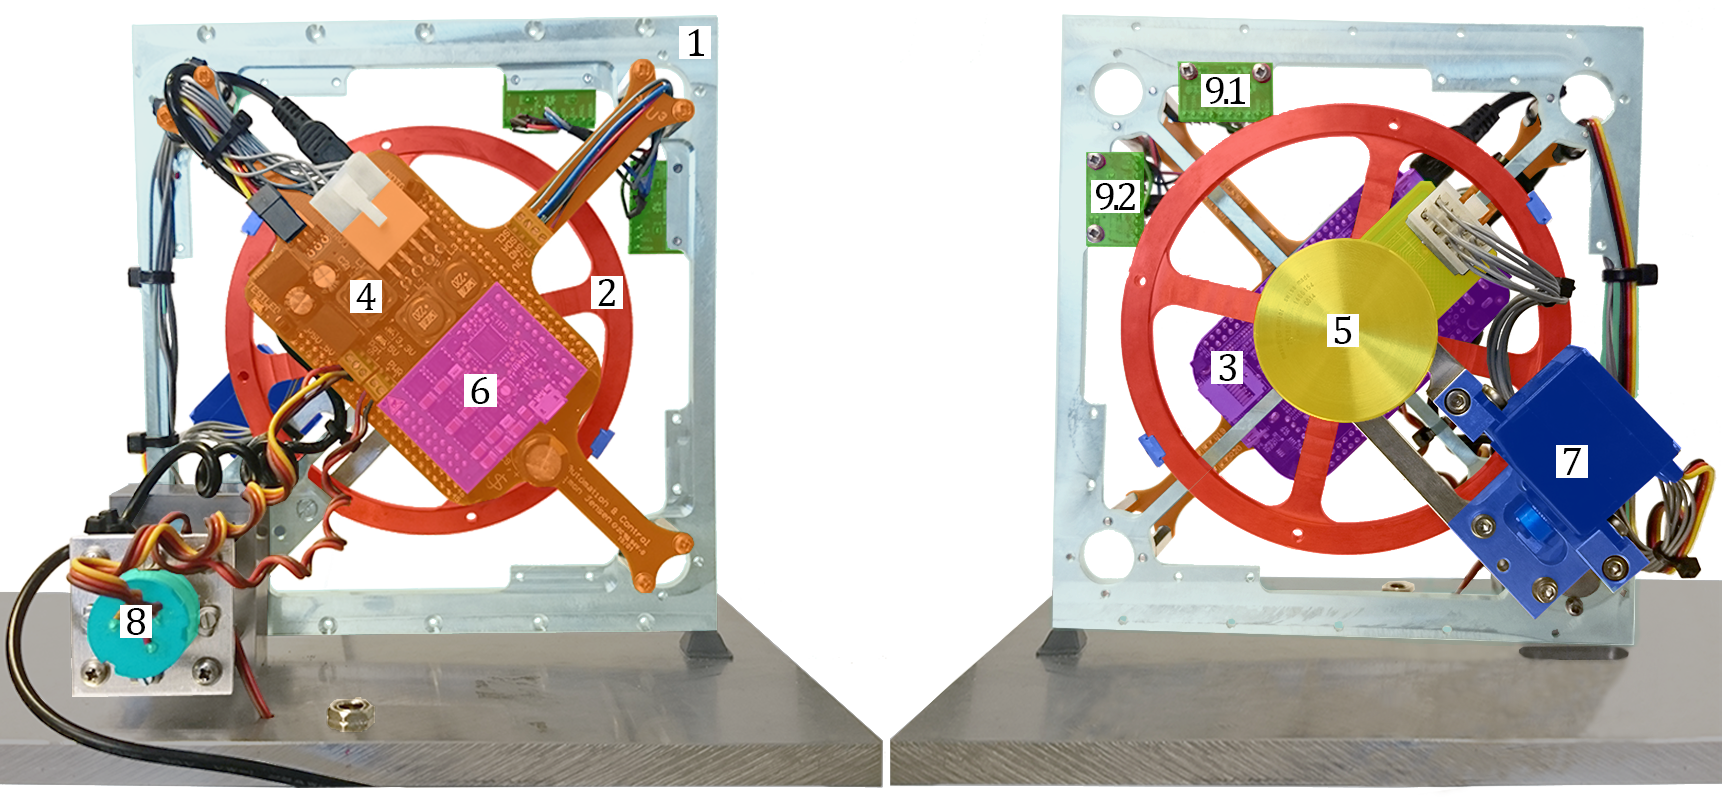
\includegraphics[scale=0.65]{Pictures/Cubli12.png}
%  \end{figure}
%\end{frame}

% ---------------------------------------------------
\section{System Description}

\begin{frame}{System Description}{Overview}

\begin{textblock*}{15cm}(2.5cm,2.5cm)
	  	%\centering
	  	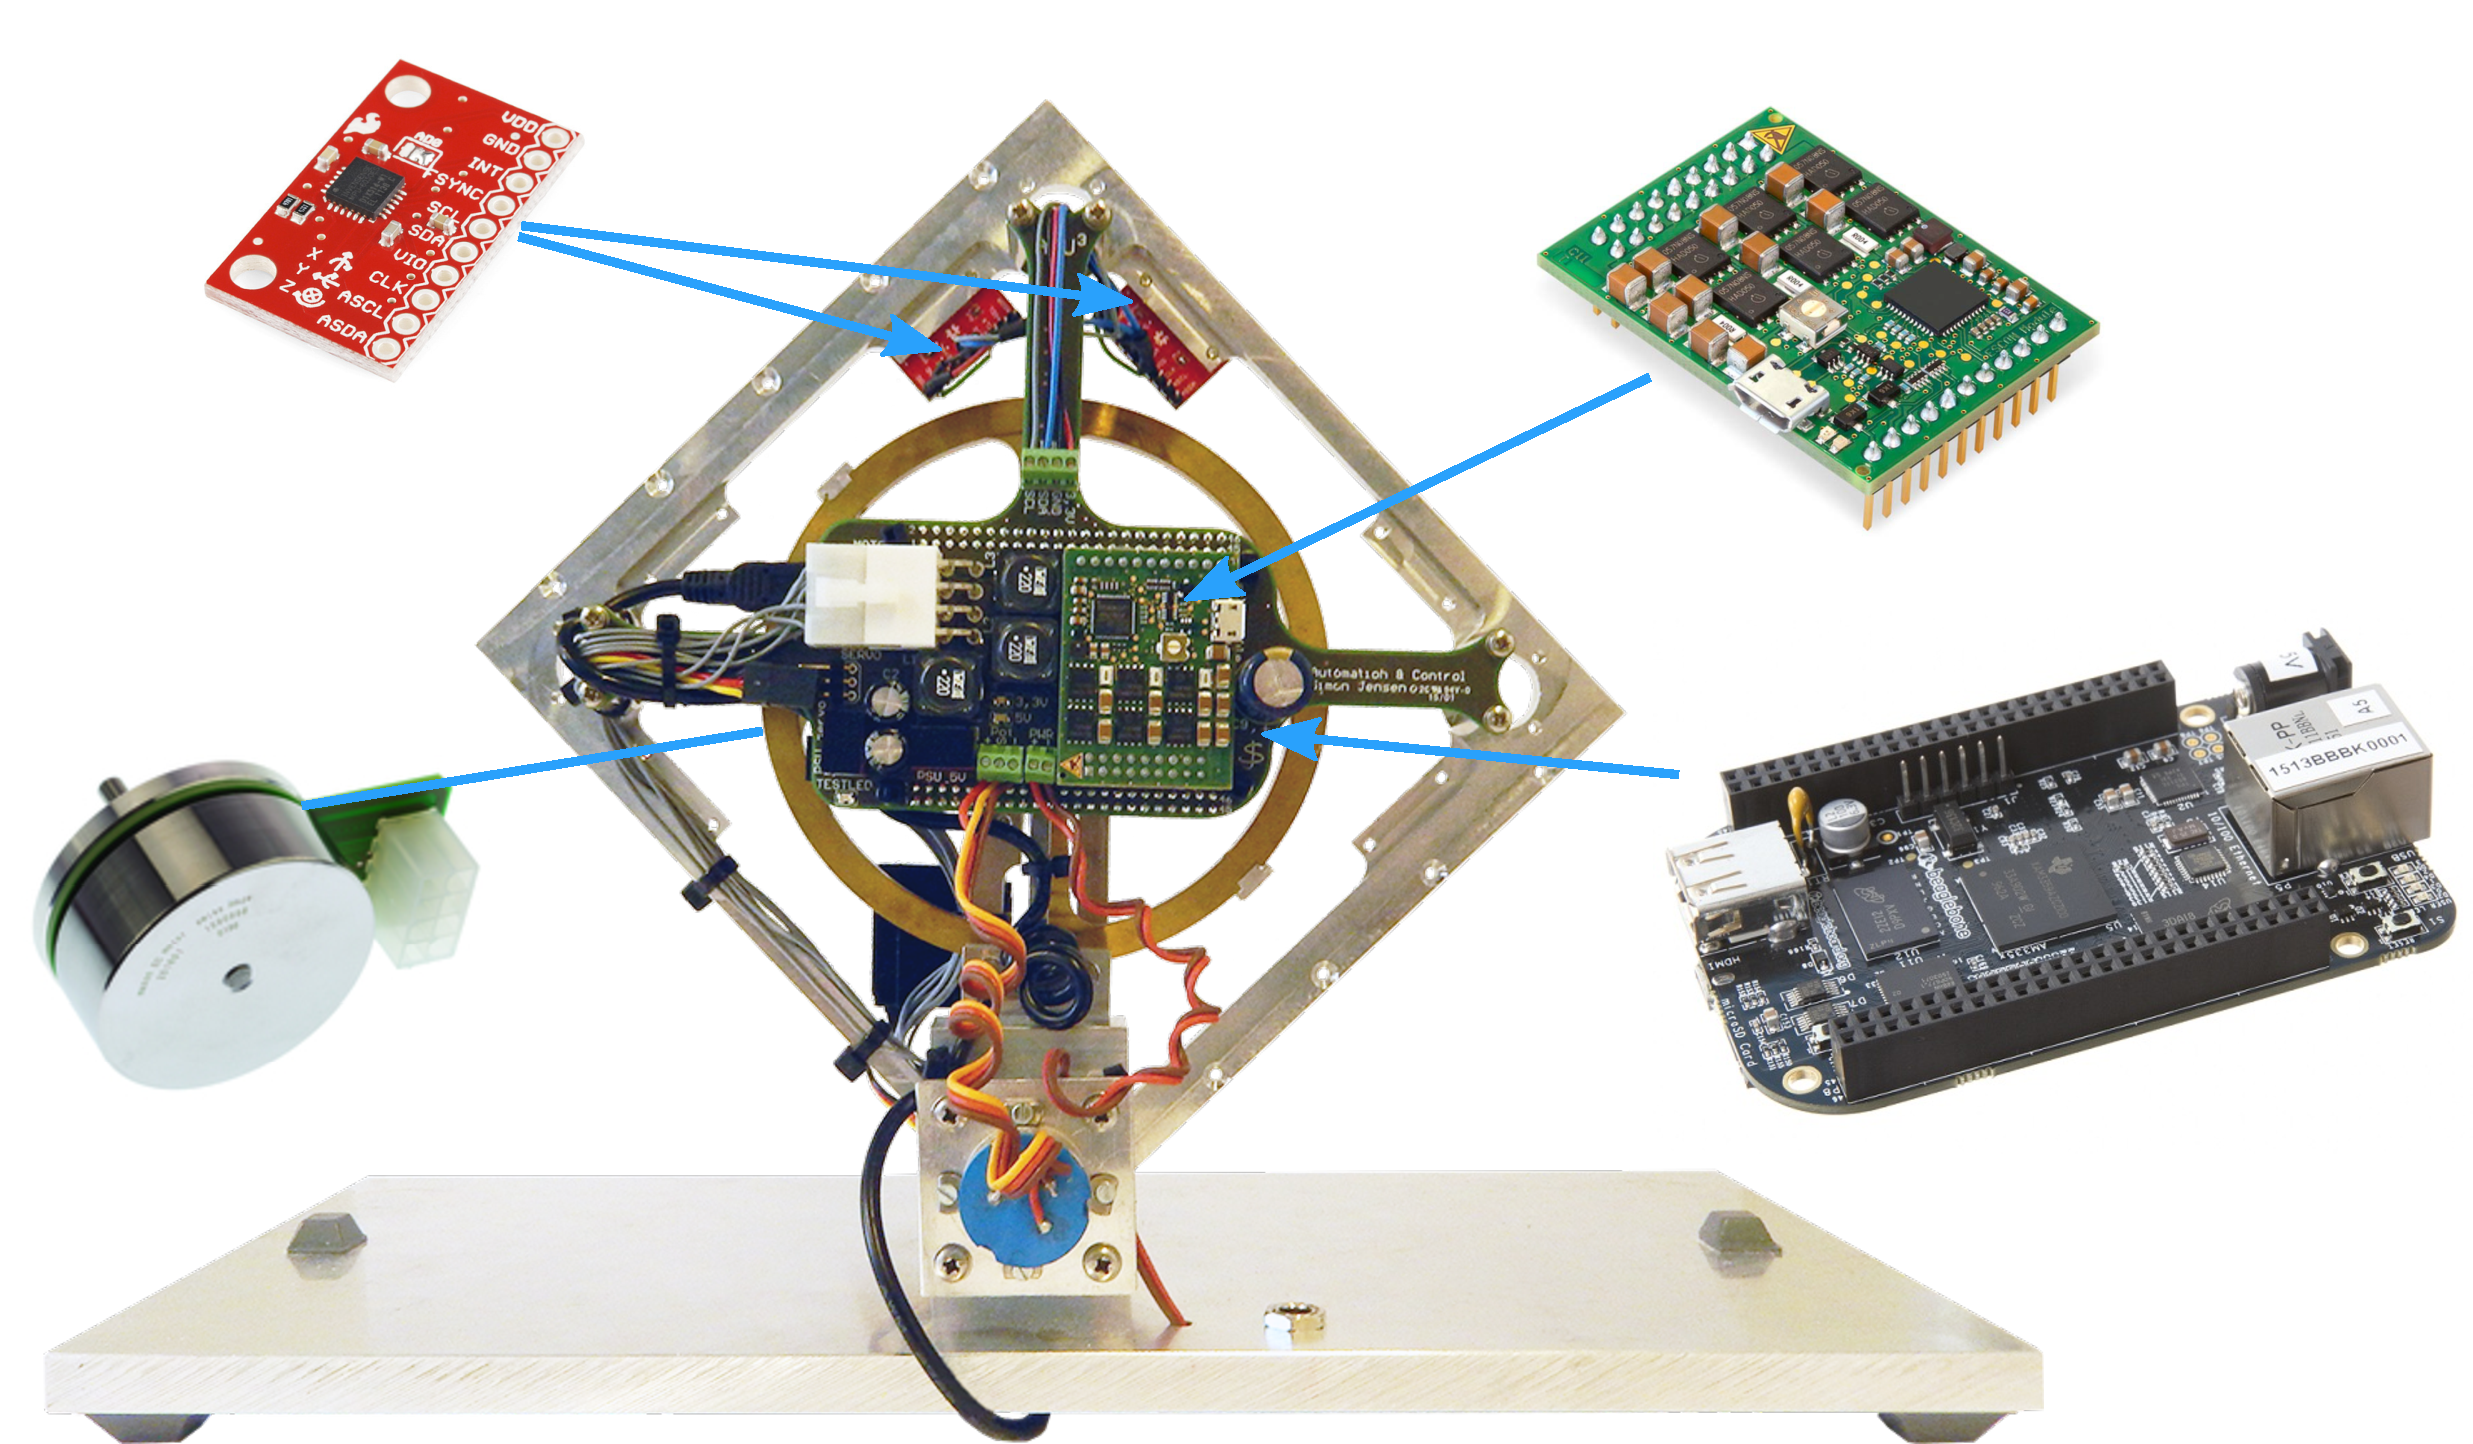
\includegraphics[scale=0.235]{Pictures/sysDescribtionTotal.pdf}
\end{textblock*}
	  
%  \begin{minipage}{\linewidth}
%  	\begin{minipage}{0.45\linewidth}
%  		\begin{figure}[H]
%  			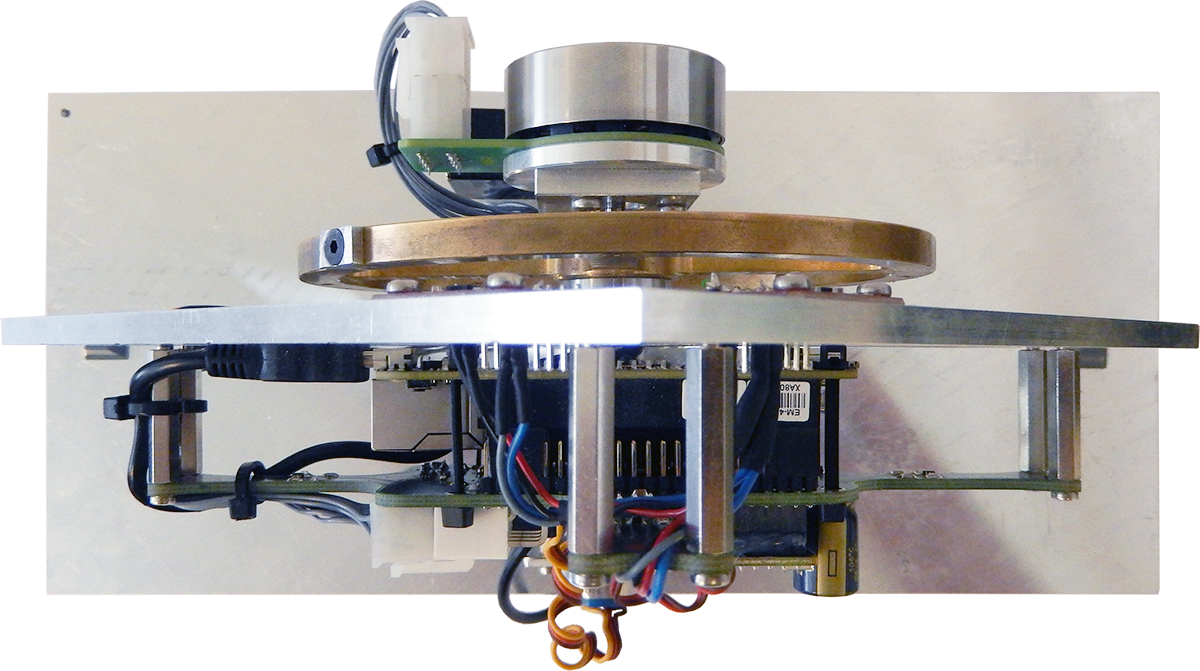
\includegraphics[scale=0.5]{Pictures/Cubli-3.png}
%  			\centering
%  		\end{figure}
%  	\end{minipage}
%  	\hspace{0.03\linewidth}
%  	\begin{minipage}{0.45\linewidth}
%  		\begin{figure}[H]
%  			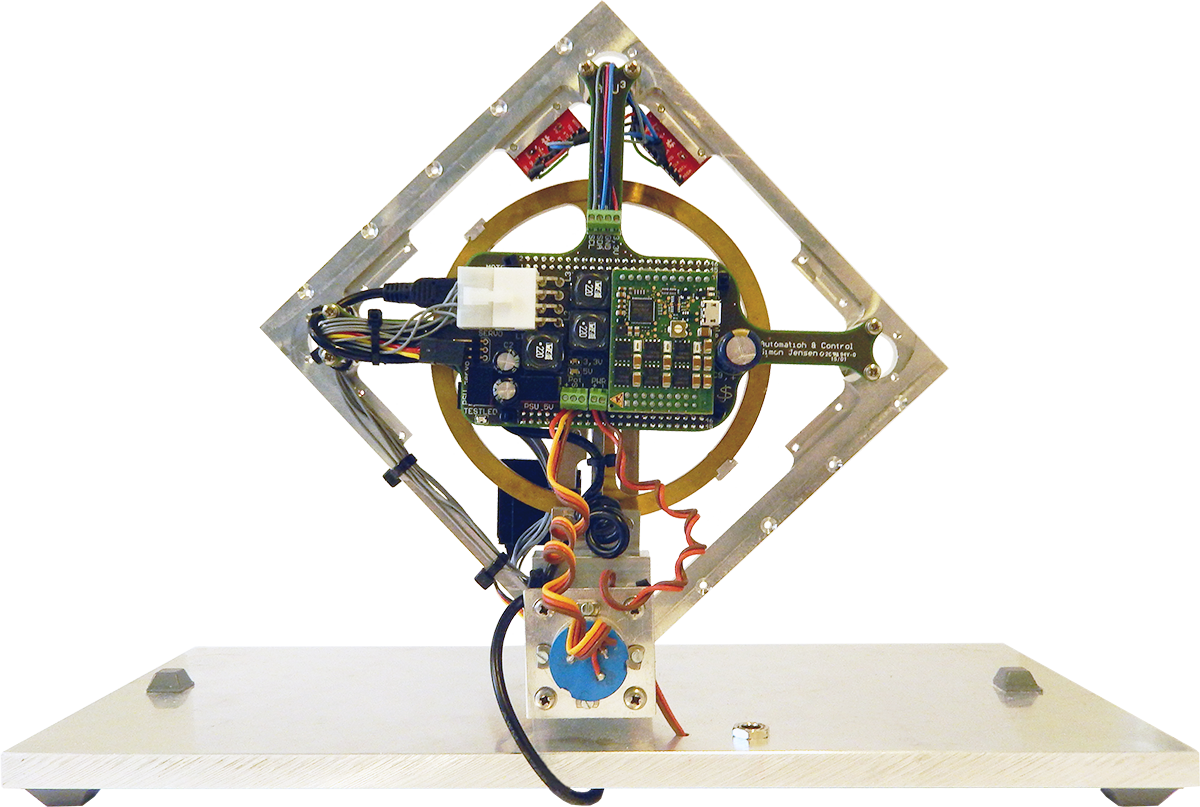
\includegraphics[scale=0.5]{Pictures/Cubli-1.png}
%  			\centering
%  		\end{figure}
%  	\end{minipage}
%  \end{minipage}
%  
%  \begin{textblock*}{8cm}(4cm,2cm)
%  	%\centering
%  	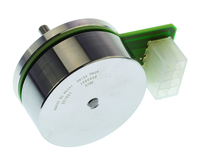
\includegraphics[scale=0.30]{Pictures/EC45FL.jpg}
%  \end{textblock*}
%  
%\begin{textblock*}{8cm}(4cm,7cm)
%	%\centering
%	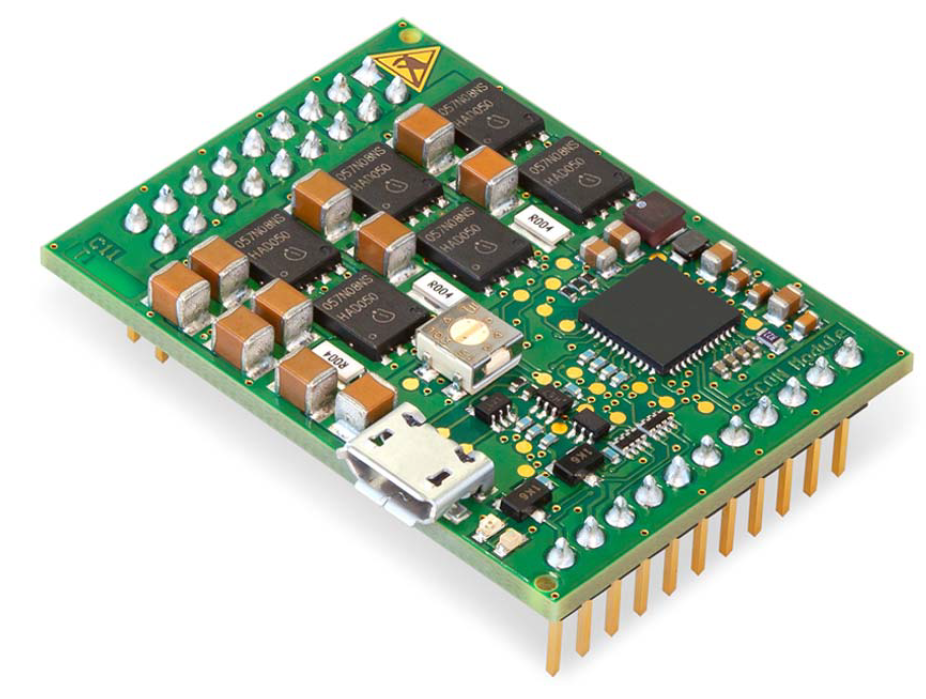
\includegraphics[scale=0.08]{Pictures/esconMotorControl.png}
%\end{textblock*}
%
%\begin{textblock*}{8cm}(8cm,7.5cm)
%	%\centering
%	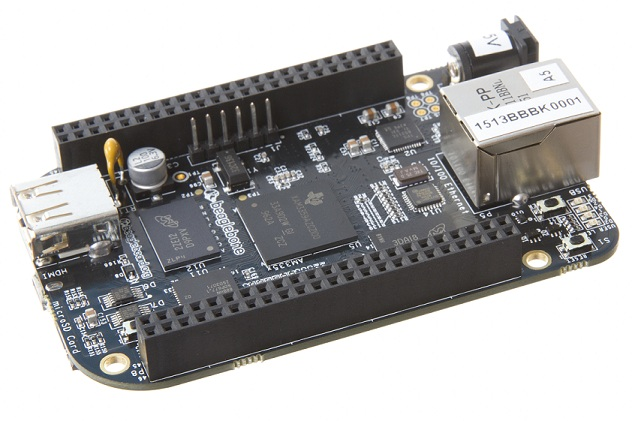
\includegraphics[scale=0.40]{Pictures/beagleBoneBlack.jpg}
%\end{textblock*}

\end{frame}

%\begin{frame}{System Description}{Overview}
%	\begin{figure}[H]
%		\centering
%		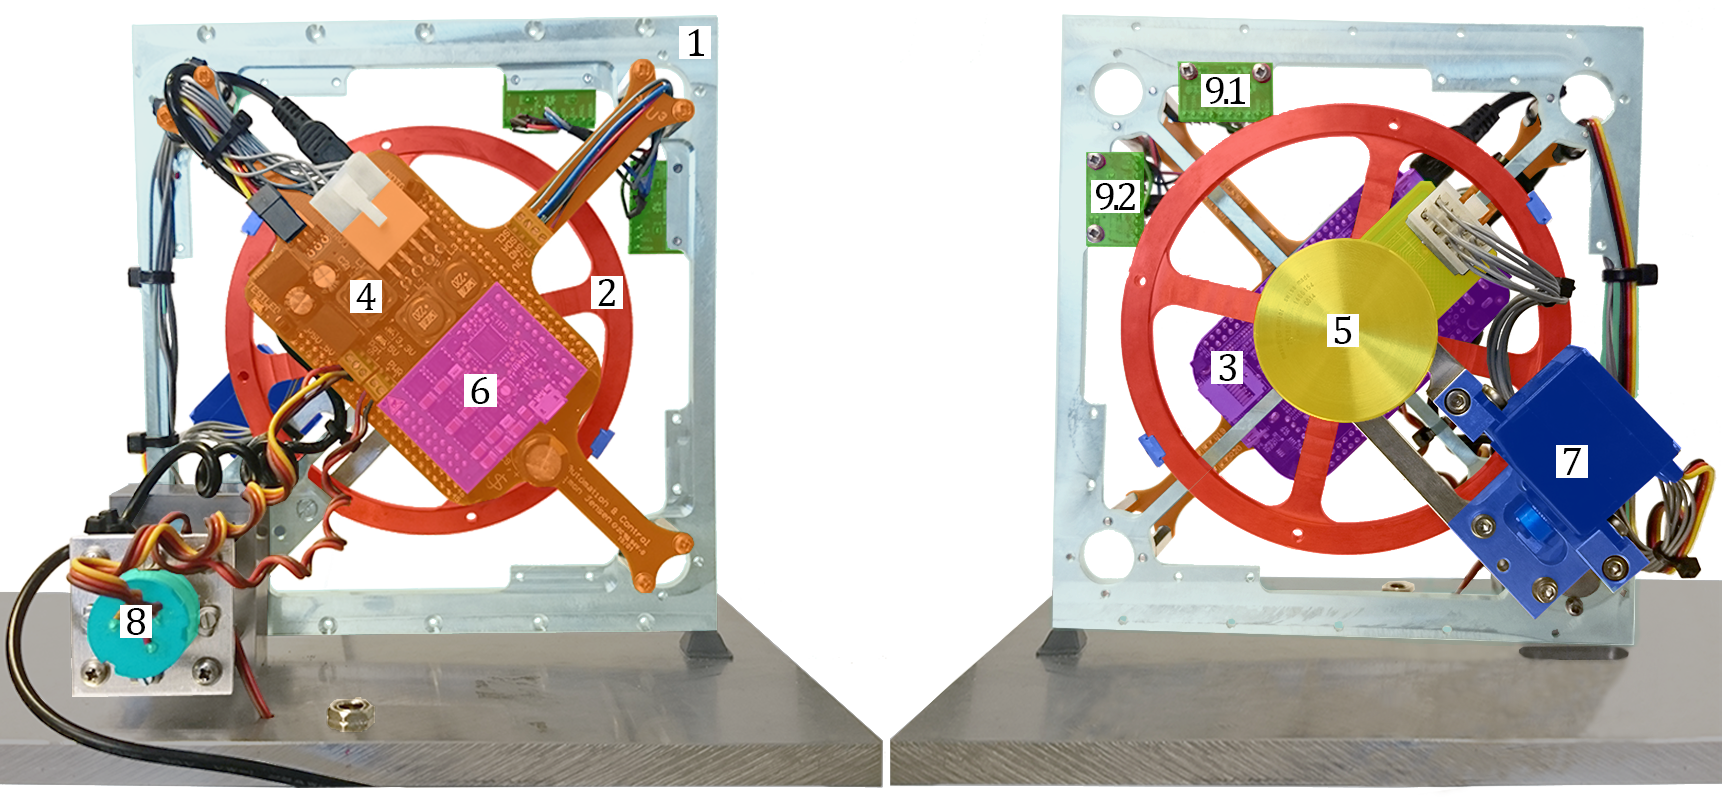
\includegraphics[scale=0.16]{Pictures/Cubli12.png}
%	\end{figure}
%\end{frame}

% -------------------------------------------------------
\section{Requirements}

\begin{frame}{Requirements}{Design Considerations}
	
	\begin{figure}[H]
		
\includegraphics[scale=0.4]{Pictures/reqCubli0rad.png}
		\centering
	\end{figure}
	
\begin{itemize}
 \item {Balancing at \si{\theta_F} =  0 rad}
 \linebreak
%  \begin{itemize}
%	%\item {Starting out from equilibrium position at null velocity}
%	\item {Starting with the wheel at \si{0\ rad/s}}
%	\linebreak
%	\end{itemize}
\item {Still balance with changing angles of the baseplate}
\end{itemize}


\end{frame}

% -----------------------------------------------------------------
\section{Model}
\subsection{Overview}
\begin{frame}{Model}{Overview}
	\begin{figure}[H]
		\centering
		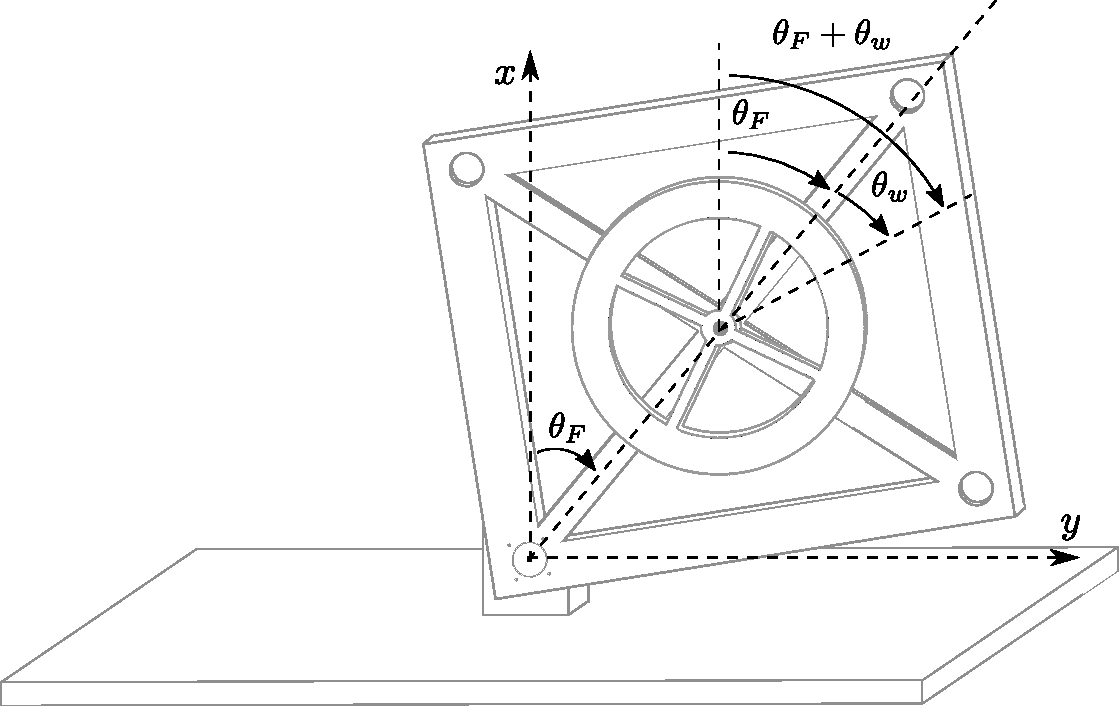
\includegraphics[scale=0.5]{Pictures/mechanicalSystem.pdf}
	\end{figure}
\end{frame}

\subsection{Free-Body Diagram}
\begin{frame}{Model}{Free-Body Diagram of the Wheel}
	\begin{textblock*}{15cm}(5cm,2cm)
		%\centering
		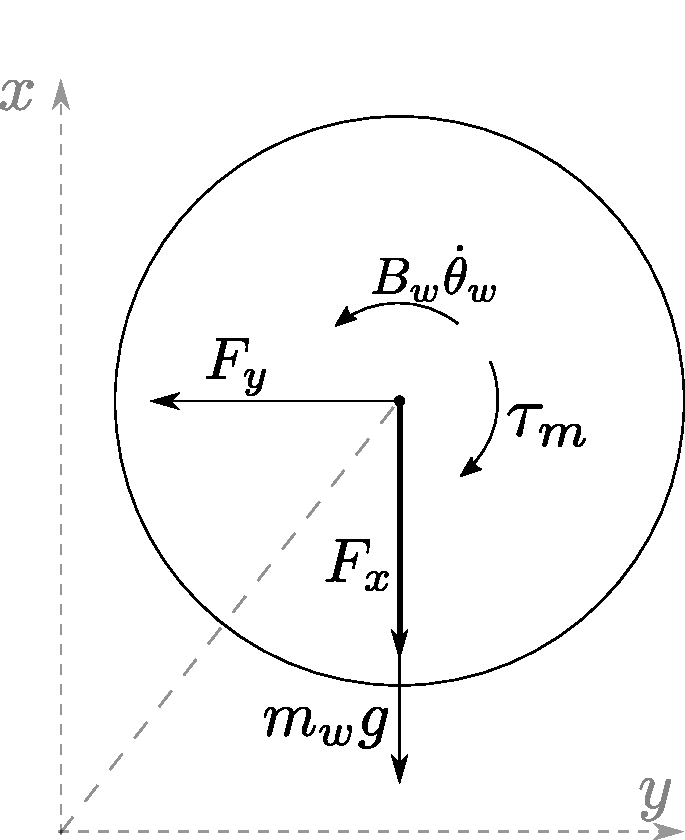
\includegraphics[scale=0.40]{Pictures/freeBodyWheel.pdf}
	\end{textblock*}
	
	\begin{textblock*}{15cm}(0cm,8cm)
	\begin{displaymath}	
	  \si{ J_w (\vec{\ddot{\theta}_F} + \vec{\ddot{\theta}_w}) =} 
	  \si{ \vec{\tau_m} - B_w \vec{\dot{\theta}_w }}
	\end{displaymath}
	\end{textblock*}
\end{frame}

\begin{frame}{Model}{Free-Body Diagram of the Frame}

%	\begin{textblock*}{5cm}(3cm,1cm) % {block width} (coords)
%		\includegraphics[width=5cm]{images/logo.jpg}
%	\end{textblock*}
	\only<1-2>{
	\begin{textblock*}{15cm}(5cm,2cm)
		%\centering
		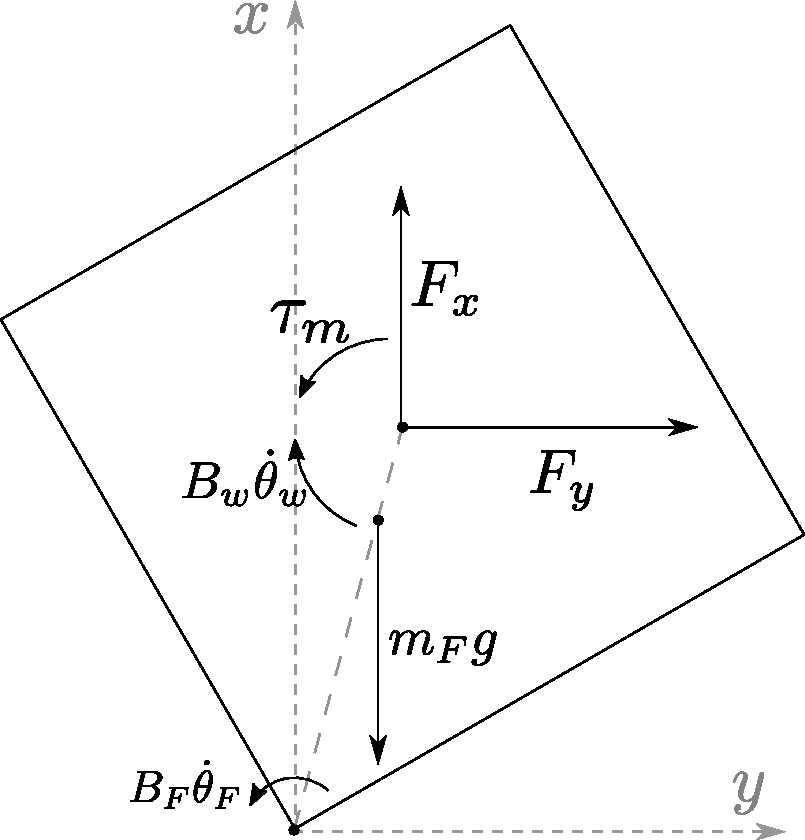
\includegraphics[scale=0.40]{Pictures/freeBodyFrame.pdf}%
	\end{textblock*}
	}
	\only<1| handout:1>{
	\begin{textblock*}{15cm}(0cm,8cm)
	\begin{displaymath}
	\si{J_F \vec{\ddot{\theta}_F} =}
	\si{-B_F \vec{\dot{\theta}_F} + \vec{l_F} \times (m_F\cdot \vec{g}) + \vec{l_w} \times \vec{F} - \vec{\tau_m} + B_w \vec{\dot{\theta}_w}}
	\end{displaymath}
	\end{textblock*}
	
}
	\only<2| handout:2>{
		\begin{textblock*}{15cm}(0cm,8cm)
		\begin{displaymath}
		\si{ \vec{l_w} \times \vec{F} = (-{l_w}^2 \cdot m_w \ddot{\theta}_F + l_w\ sin(\theta_F)\ m_w \cdot g ) \cdot \hat{k}} %\nonumber
		\end{displaymath}
		\end{textblock*}
	}

\end{frame}

%\begin{frame}{Model}{Construction}
%	
%		\begin{flalign}
%		\si{\vec{l_w} \times \vec{F}}	\nonumber
%		\end{flalign}
%		
%		\begin{flalign}
%		\si{\vec{l_w} \times \vec{F}} &=
%		\begin{vmatrix}
%		\ \si{\vec{\hat{i}}} \nonumber               & \si{\vec{\hat{j}}} \nonumber              & \si{\vec{\hat{k}}}\nonumber \ \ \ \\ 
%		\ \si{ l_w \cdot cos( \theta_F ) }\nonumber  & \si{ l_w \cdot sin( \theta_F ) }\nonumber & 0 \nonumber                 \ \ \ \\ 
%		\ \si{ F_x }      \nonumber                  & \si{ F_y }      \nonumber                & 0      \nonumber            \ \ \  
%		\end{vmatrix}\nonumber
%		\end{flalign}
%	
%%		\begin{flalign}
%%		\si{ \vec{l_w} \times \vec{F} = (-{l_w}^2 \cdot m_w \ddot{\theta}_F + l_w\ sin(\theta_F)\ m_w \cdot g ) \cdot \hat{k}} \nonumber
%%		\end{flalign}
%%	
%	
%\end{frame}

\subsection{Frame Angle and Wheel velocity}
\begin{frame}{Model}{Frame and Wheel Equations}
	\begin{itemize}
		\item Acceleration of the frame
	\end{itemize}
\small
	\begin{flalign}
%	 \si{\ddot{\theta}_F =} &\si{ -\frac{B_F}{J_F + m_w \cdot {l_w}^2} \cdot \dot{\theta}_F + \frac{(m_F \cdot l_F + m_w \cdot l_w) \cdot g}{J_F + m_w \cdot {l_w}^2} \cdot sin(\theta_F) }& \nonumber \\ 
%		&\si{- \frac{1}{J_F + m_w \cdot {l_w}^2} \cdot \tau_m + \frac{B_w}{J_F + m_w \cdot {l_w}^2} \cdot \dot{\theta}_w} & \nonumber
\si{\ddot{\theta}_F = \frac{- B_F \cdot \dot{\theta}_F + (m_F \cdot l_F + m_w \cdot l_w) \cdot g \cdot sin(\theta_F) - \tau_m + B_w \cdot \dot{\theta}_w}{J_F + m_w \cdot {l_w}^{2}}} \nonumber
	\end{flalign}
	\vspace{0.5cm}
\normalsize	
%
\begin{itemize}
	\item Acceleration of the wheel
\end{itemize}
\small
	\begin{flalign}
%	\si{\ddot{\theta}_w =} &\si{\frac{J_w+J_F+m_w \cdot {l_w}^{2}}{J_w \cdot (J_F+m_w \cdot {l_w}^{2})} \cdot \tau_m - \frac{(J_w+J_F+{l_w}^{2} \cdot m_w) \cdot B_w}{J_w \cdot (J_F+m_w \cdot  {l_w}^2)} \cdot \dot{\theta}_w}& \nonumber \\
%	&\si{ - \frac{(m_F \cdot l_F + m_w \cdot l_w) \cdot g}{J_F+m_w \cdot {l_w}^{2}} \cdot sin(\theta_F) + \frac{B_F}{J_F+m_w \cdot {l_w}^{2}} \cdot \dot{\theta}_F} & \nonumber
\si{\ddot{\theta}_w = \frac{\tau_m - B_w \cdot \dot{\theta}_w}{J_w} - \ddot{\theta}_F} \nonumber
	\end{flalign}
\normalsize
	
\end{frame}

\subsection{Linearization}
\begin{frame}{Model}{Linearization}
%	\begin{flalign}
%	\si{\ddot{\theta}_F =} &\si{ -\frac{B_F}{J_F + m_w \cdot {l_w}^2} \cdot \dot{\theta}_F + \frac{(m_F \cdot l_F + m_w \cdot l_w) \cdot g}{J_F + m_w \cdot {l_w}^2} \cdot sin(\theta_F) }& \nonumber \\ 
%	&\si{- \frac{1}{J_F + m_w \cdot {l_w}^2} \cdot \tau_m + \frac{B_w}{J_F + m_w \cdot {l_w}^2} \cdot \dot{\theta}_w} & \nonumber
%	\end{flalign}
\small
\begin{flalign}
\si{(J_F+m_w \cdot {l_w}^{2})\cdot (\ddot{\theta}_{F})} &= \si{- B_F \cdot (\dot{\theta}_{F})}   \nonumber\\
&\ \ \ \ \si{+ (m_F \cdot l_F + m_w \cdot l_w) \cdot g \cdot sin(\theta_{F})} \nonumber\\
&\ \ \ \ \si{- (\tau_{m}) + B_w \cdot (\dot{\theta}_{w})} \nonumber
%	\si{(J_F+m_w \cdot {l_w}^{2}) (\ddot{\theta}_{F_0} + \Delta \ddot{\theta}_F )= f( (\dot{\theta}_{F_0} + \Delta \dot{\theta}_F), \ (\theta_{F_0} + \Delta \theta_F), \ (\tau_{m_0} + \Delta \tau_m),\  (\dot{\theta}_{w_0} + \Delta \dot{\theta}_w) ) } \nonumber
\end{flalign}
\normalsize

\pause
	\begin{itemize}
		\item {Operating point} 
		\begin{itemize}
			\item {\si{\theta_{F_0}\ =\ 0\ rad}}
			\item {\si{\dot{\theta}_{w_0}\ =\ 0\ rad \cdot s^{-1}}}
			\item {variation around operating point is \si{\Delta \theta_F}}
		\end{itemize}
	\end{itemize}
	
	\pause
	\small
	\begin{flalign}
	\si{(J_F+m_w \cdot {l_w}^{2})\cdot(\ddot{\theta}_{F_0} + \Delta \ddot{\theta}_F )} &= \si{- B_F \cdot (\dot{\theta}_{F_0} + \Delta \dot{\theta}_F) }   \nonumber\\
	&\ \ \ \ \si{+ (m_F \cdot l_F + m_w \cdot l_w) \cdot g \cdot sin(\theta_{F_0} + \Delta \theta_F)} \nonumber\\
	&\ \ \ \ \si{- (\tau_{m_0} + \Delta \tau_m) + B_w \cdot (\dot{\theta}_{w_0} +\Delta \dot{\theta}_w)} \nonumber
%	\si{(J_F+m_w \cdot {l_w}^{2}) (\ddot{\theta}_{F_0} + \Delta \ddot{\theta}_F )= f( (\dot{\theta}_{F_0} + \Delta \dot{\theta}_F), \ (\theta_{F_0} + \Delta \theta_F), \ (\tau_{m_0} + \Delta \tau_m),\  (\dot{\theta}_{w_0} + \Delta \dot{\theta}_w) ) } \nonumber
	\end{flalign}
	\normalsize
	
\end{frame}

\begin{frame}{Model}{Linearization}
		\small
		\begin{flalign}
		\si{(J_F+m_w \cdot {l_w}^{2}) \Delta \ddot{\theta}_F } &= \cancelto{0}{\si{f( \dot{\theta}_{F_0}, \ \theta_{F_0}, \ \tau_{m_0},\ \dot{\theta}_{w_0} )}}   \nonumber\\
		&\ \ \ \ \si{+ \frac{\partial}{\partial \dot{\theta}_F} f\cdot \Delta \dot{\theta}_F + \frac{\partial}{\partial \theta_F} f\cdot \Delta \theta_F + \frac{\partial}{\partial \tau_m} f\cdot \Delta \tau_m + \frac{\partial}{\partial \dot{\theta}_w} f\cdot \Delta \dot{\theta}_w} \nonumber
		\end{flalign}
		\normalsize
		\begin{itemize}
			\item {Linearized expression for frame acceleration}
		\end{itemize}
\small
		\begin{flalign}
%		&\si{(J_F+m_w \cdot {l_w}^{2}) \Delta \ddot{\theta}_F =} \nonumber \\
%		&\si{-B_F \Delta \dot{\theta}_F +  ( m_F \cdot l_F + m_w \cdot l_w ) \cdot g \cdot \Delta \theta_F - \Delta \tau_m + B_w \Delta \dot{\theta}_w } \nonumber
		\si{(J_F+m_w \cdot {l_w}^{2}) \Delta \ddot{\theta}_F = -B_F \Delta \dot{\theta}_F +  ( m_F \cdot l_F + m_w \cdot l_w ) \cdot g \cdot \Delta \theta_F - \Delta \tau_m + B_w \Delta \dot{\theta}_w } \nonumber
		\end{flalign}
		\normalsize
\end{frame}

\subsection{Block Diagram}
\begin{frame}{Model}{Block Diagram}
	
		\begin{itemize}
			\item {Laplace Transformation}
			\begin{itemize}
				\item {Replace \si{\theta_w}}
			\end{itemize}
		\end{itemize}
		\small
		\begin{flalign}
		&\si{\theta_w\cdot s^2 = \frac{\tau_m - B_w \theta_w\cdot s}{J_w} - \theta_F\cdot s^2} \nonumber \\\nonumber\\
		%\si{{\theta}_w \cdot s^2 = \frac{\tau_m - B_w \cdot {\theta}_w\cdot s }{J_w} - {\theta}_F \cdot s^2} \nonumber
		&\si{(J_F+m_w \cdot {l_w}^{2}) \cdot \theta_F \cdot s^2 = -B_F \theta_F\cdot s +  ( m_F \cdot l_F + m_w \cdot l_w ) g \cdot \theta_F - \tau_m + B_w \theta_w\cdot s } \nonumber
		\end{flalign}
		\normalsize
	
	\begin{figure}[H]
		\centering
		  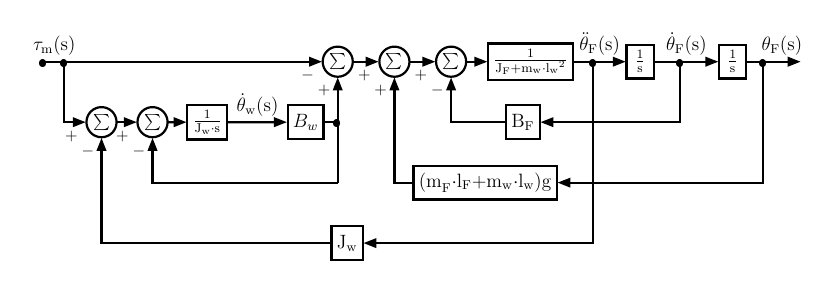
\begin{tikzpicture}[ auto,
                       thick,                         %<--setting line style
                       node distance=1.5cm,             %<--setting default node distance
                       scale=0.48,                     %<--|these two scale the whole thing
                       every node/.style={scale=0.58}, %<  |(always change both)
                       >/.tip={Triangle[angle=40:5pt]}
                       ]

    %-- Blocks creation --%
    \draw
      % DIRECT TERM %
      node[shape=coordinate][](input1) at (0,0){}
      node[shape=coordinate][](feedForward) at (0.5,0){}
      node(sum1) at (7.75,0) [sum] {\si{\sum}}
      node(sum2) at (9.25,0) [sum]{\si{\sum}}
      node(sum3) at (10.75,0) [sum]{\si{\sum}}

      node(torque2rotacc1) at (12.85,0) [block]{\large \si{\frac{1}{J_F + m_w \cdot {l_w}^{2}}}}

      node(integration1) at (15.75,0) [block] {\large \si{\frac{1}{s}}}
      node(integration2) at (18.2,0) [block] {\large \si{\frac{1}{s}}}

      node[shape=coordinate][](output) at (19,0){}
      node[shape=coordinate][](veloFeedbackNode) at (16.8,0){}
      node[shape=coordinate][](accFeedbackNode) at (14.5,0){}
    ;
    \draw
      % REACTION WHEEL EQUATIONS %  
      node(sum4) at (1.5,-1.6) [sum]{\si{\sum}}
      node(sum5) at (2.85,-1.6) [sum]{\si{\sum}}

      node(torque2rotacc2) at (4.3,-1.6) [block]{\large \si{\frac{1}{J_w \cdot s}}}
      % node(integration3) [block, right of = torque2rotacc2] {$\frac{1}{s}$}
      node(frictionWheel) at (6.9,-1.6) [block] {\large $B_w$}

      node[shape=coordinate][](veloWheelFeedback) at (7.75,-3.2){}
    ;
    \draw
      % FEEDBACKS %
      node(accFeedback) at (8, -4.8) [block] {\large \si{J_w}}
      node(veloFeedback) at (12.65,-1.6) [block] {\large \si{B_F}}
      node(angleFeedback) at (11.65,-3.2) [block] {\large \si{(m_F \cdot l_F + m_w \cdot l_w)g}}
    ;
    %-- Block linking --%
    % INPUT %
    \draw[-](input1)        -- node{\large \si{\tau_m(s)}}(feedForward);
    \draw[->](feedForward)  -- (sum1);

    % OUTPUT %
    \draw[-](integration2)  -- (output);
    \draw[->](output)       -- node {\large \si{\theta_{F}(s)}} (20,0);

    % DIRECT TERM %
    \draw[->] (sum1)            -- (sum2);
    \draw[->] (sum2)            -- (sum3);
    \draw[->] (sum3)            -- (torque2rotacc1);
    \draw[->] (torque2rotacc1)  -- node{\large \si{\ddot{\theta}_F(s)}}(integration1);
    \draw[->] (integration1)    -- node{\large \si{\dot{\theta}_F(s)}}(integration2);

    % REACTION WHEEL EQUATIONS %
    \draw[->] (feedForward)     |- (sum4);
    \draw[->] (sum4)            -- (sum5);
    \draw[->] (sum5)            -- (torque2rotacc2);
    \draw[->] (torque2rotacc2)  -- node{\large \si{\dot{\theta}_w(s)}}(frictionWheel);
    % \draw[->] (integration3)    -- (frictionWheel);
    \draw[->] (frictionWheel)   -| (sum1);

    \draw[-] (frictionWheel)       -| (veloWheelFeedback);
    \draw[->] (veloWheelFeedback)  -| (sum5);

    % FEEDBACKS
    \draw[->] (accFeedbackNode)  |- (accFeedback);
    \draw[->] (accFeedback)      -| (sum4);

    \draw[->] (output)           |- (angleFeedback);
    \draw[->] (angleFeedback)    -| (sum2);

    \draw[->] (veloFeedbackNode) |- (veloFeedback);
    \draw[->] (veloFeedback)     -| (sum3);

    %-- Nodes --%
    \draw%--------------------------------------------------------------
      node at (input1)            [shift={(-0.04, -0.05 )}] {\large \textbullet}
      node at (output)            [shift={( 0.007, -0.05 )}] {\large \textbullet}
      node at (veloFeedbackNode)  [shift={( 0.007, -0.05 )}] {\large \textbullet}
      node at (accFeedbackNode)   [shift={( 0.007, -0.05 )}] {\large \textbullet}
      node at (feedForward)       [shift={( 0.007, -0.05 )}] {\large \textbullet}
      node at (frictionWheel)     [shift={( 0.70, -0.04 )}] {\large \textbullet}
    ;

    %-- Summation signs --%
      \draw%--------------------------------------------------------------
      node at (sum1) [right = -6.6mm, below = .6mm] {$-$}
      node at (sum1) [right = -3mm, below = 3.9mm]  {$+$} 
      node at (sum2) [right = -6.6mm, below = .6mm] {$+$}
      node at (sum2) [right = -3mm, below = 3.9mm]  {$+$}
      node at (sum3) [right = -6.6mm, below = .6mm] {$+$}
      node at (sum3) [right = -3mm, below = 3.9mm]  {$-$}
      node at (sum4) [right = -6.6mm, below = .6mm] {$+$}
      node at (sum4) [right = -3mm, below = 3.9mm]  {$-$}
      node at (sum5) [right = -6.6mm, below = .6mm] {$+$}
      node at (sum5) [right = -3mm, below = 3.9mm]  {$-$}
    ;

  \end{tikzpicture}
	\end{figure}
\end{frame}
%\section{Hardware and Software}
%%%%%%%%%%%%%%%%%
%\subsection{Prototype overview}
%
%\begin{frame}{Hardware and Software}{Prototype overview}
%  \begin{figure}[H]
%	\centering
%	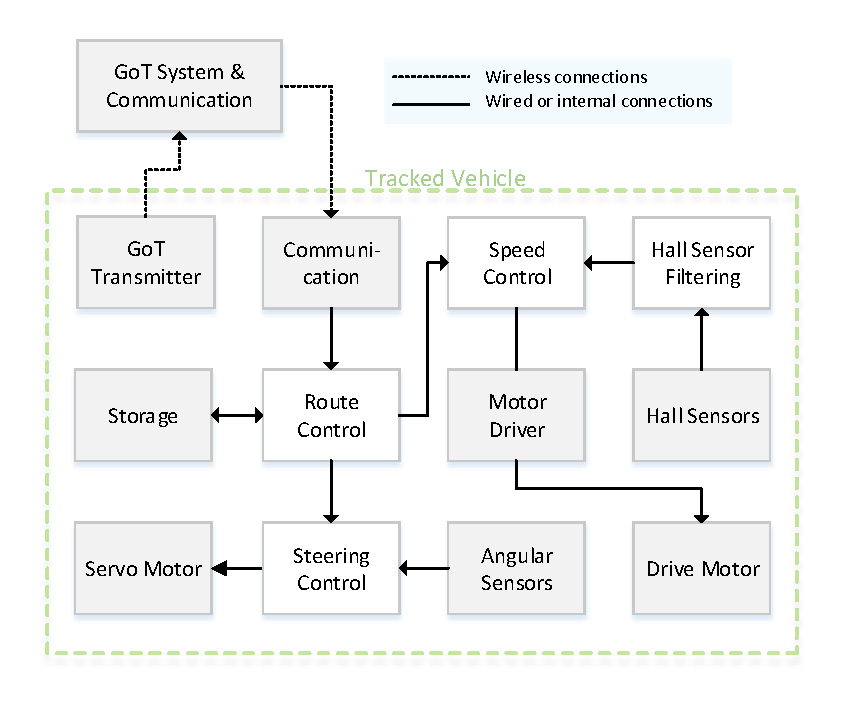
\includegraphics[scale=0.65]{Pictures/SO3.pdf}
%  \end{figure}
%\end{frame}
%%%%%%%%%%%%%%%%%
%
%%%%%%%%%%%%%%%%%
%\subsection{Hardware components}
%
%\begin{frame}{Hardware and Software}{Hardware components}
%\textbf{Controller}
%\begin{itemize}
%\item{Arduino Mega 2560}
%\end{itemize}
%  \begin{figure}[H]
%	\centering
%	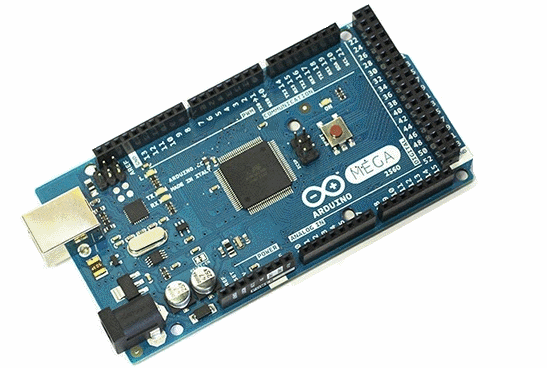
\includegraphics[scale=0.4]{Pictures/ArduinoMega.png}
%  \end{figure}
%\end{frame}
%
%\begin{frame}{Hardware and Software}{Hardware components}
%\textbf{Velocity Sensor}
%\begin{itemize}
%\item{Hall Sensor}
%\end{itemize}
%  \begin{figure}[H]
%	\centering
%	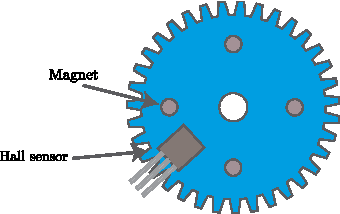
\includegraphics[scale=1.5]{Pictures/hallSensorDrawing.pdf}
%  \end{figure}
%\end{frame}
%
%\begin{frame}{Hardware and Software}{Hardware components}
%\textbf{Angular Sensor}
%\begin{itemize}
%\item{HMC5883L Magnetometer}
%\end{itemize}
%
%  \begin{minipage}{\linewidth}
%  	\begin{minipage}{0.45\linewidth}
%  		\begin{figure}[H]
%  			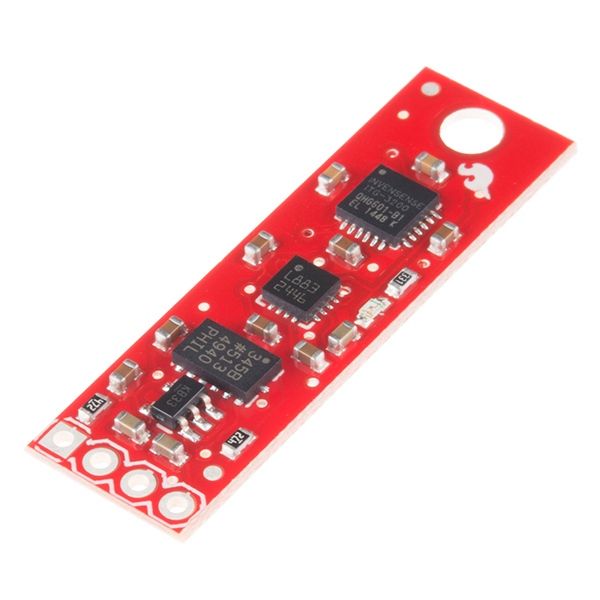
\includegraphics[scale=0.7]{Pictures/NineDegree.jpg}
%  			\centering
%  		\end{figure}
%  	\end{minipage}
%  	\hspace{0.03\linewidth}
%  	\begin{minipage}{0.45\linewidth}
%  		\begin{figure}[H]
%  			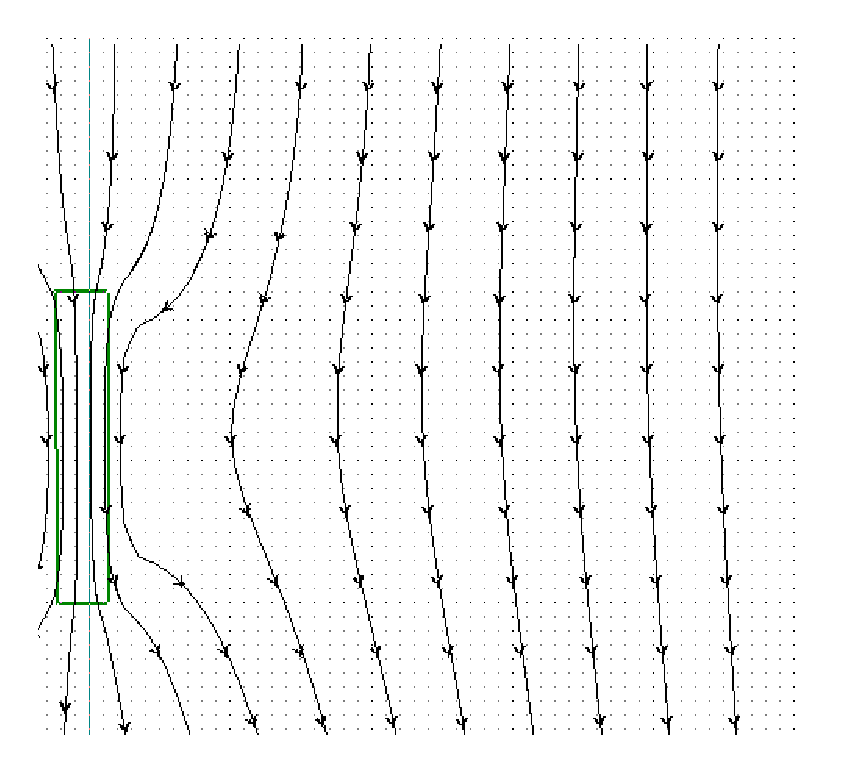
\includegraphics[scale=0.35]{Pictures/Magne.pdf}
%  			\centering
%  		\end{figure}
%  	\end{minipage}
%  \end{minipage}
%
%\end{frame}
%
%
%
%
%\begin{frame}{Hardware and Software}{Hardware components}
%\textbf{Position Sensor}
%\begin{itemize}
%\item{Games on Track system (GoT)}
%\end{itemize}
%  \begin{figure}[H]
%	\centering
%	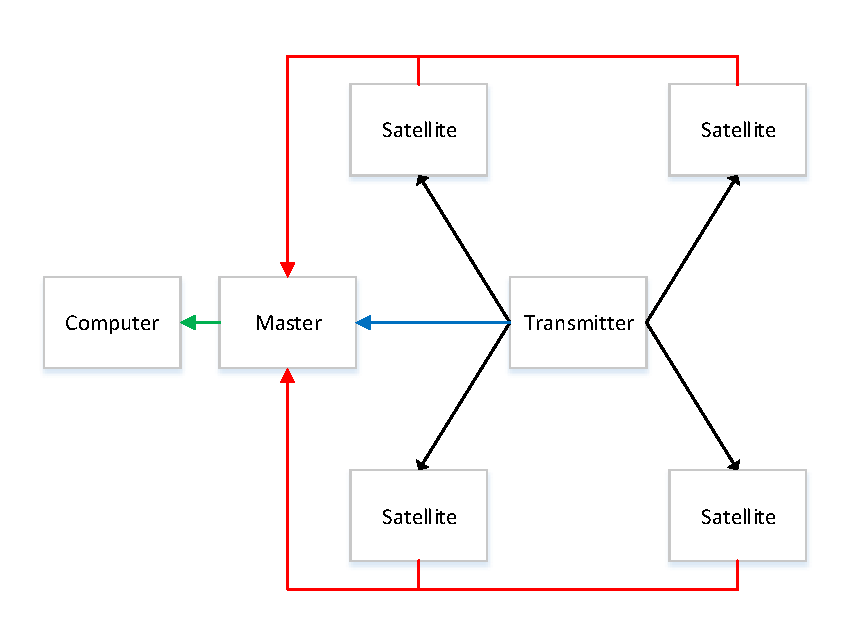
\includegraphics[scale=0.6]{Pictures/GOTNew.pdf}
%  \end{figure}
%\end{frame}
%
%\begin{frame}{Hardware and Software}{Hardware components}
%\begin{itemize}
%\item {Communication}
%\item {Storage}
%\item {Motor driver}
%\item {Battery and Power monitor}
%\end{itemize}
%\end{frame}
%%%%%%%%%%%%%%%%%
%
%%%%%%%%%%%%%%%%%
%\subsection{Software}
%
%\begin{frame}{Hardware and Software}{Software}
%\begin{itemize}
% \item {Real Time Operating System}
%  \begin{itemize}
%	\item {KRNL by Jens Dalsgaard Nielsen}
%\end{itemize}
%\end{itemize}
%
%  \begin{figure}[H]
%	\centering
%	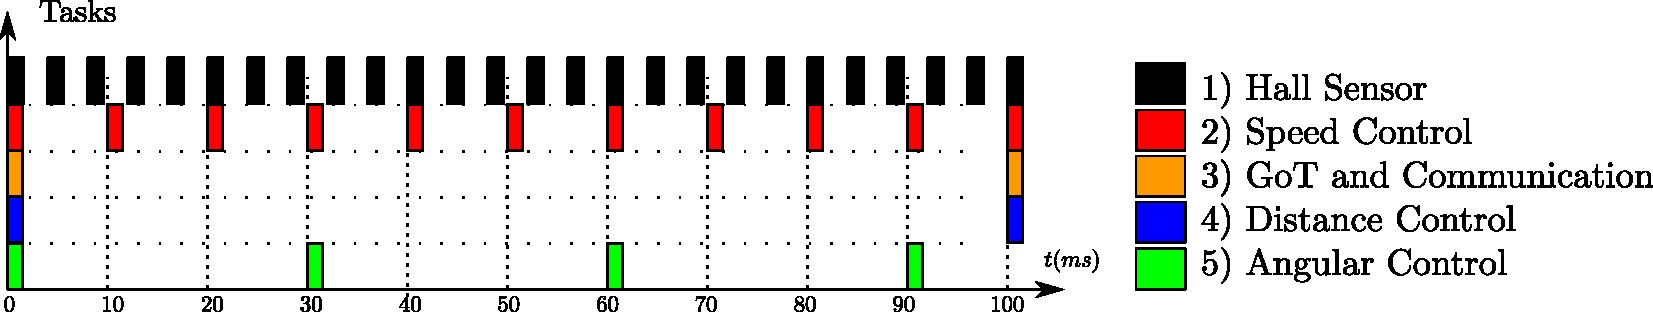
\includegraphics[scale=0.35]{Pictures/scheduleRequest.pdf}
%  \end{figure}
%
%  \begin{figure}[H]
%	\centering
%	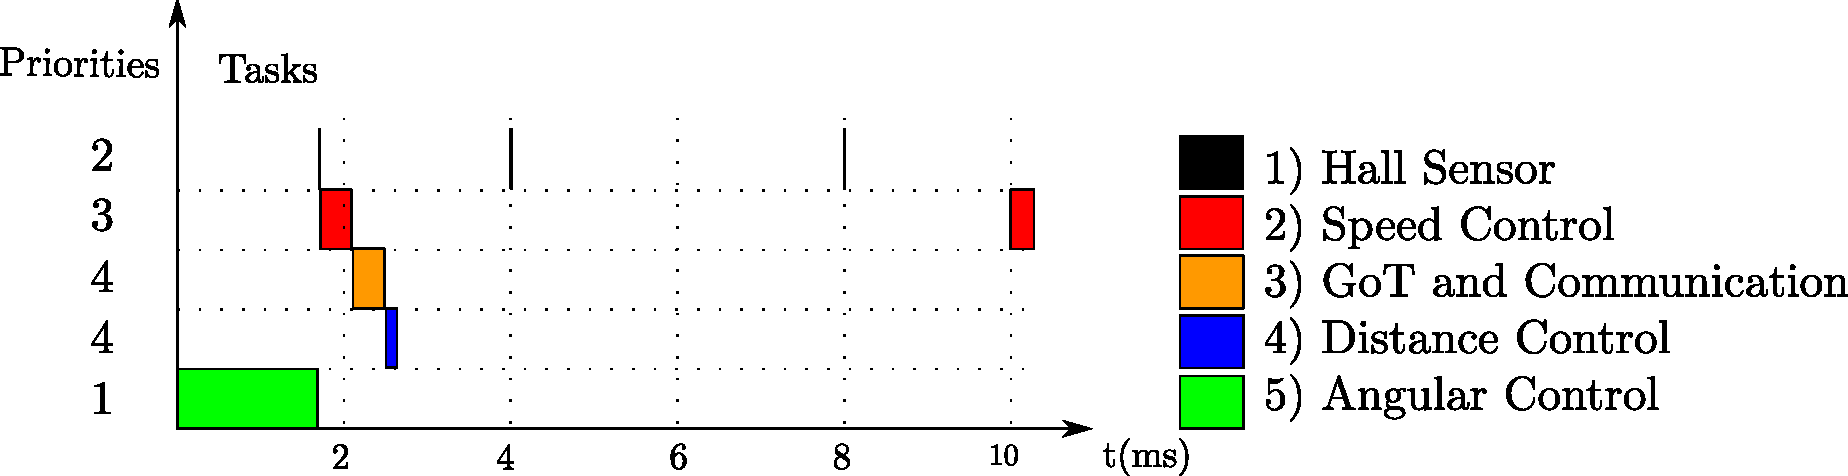
\includegraphics[scale=0.3]{Pictures/schedulePriorities.pdf}
%  \end{figure}
%\end{frame}
	%%%%%%%%%%%%%%%%%%%%%%%%%%%% Julien %%%%%%%%%%%%%%%%%%%%%%%%%%%%%
\section{Parameters}

%- 1 -%
\begin{frame}{Model Parameters}{List of Parameters}
  \begin{table}[H]\centering
  \begin{tabular}{|c|S[table-figures-exponent=1]@{\,}|s[table-unit-alignment = left]|}
    \hline
      \textbf{Parameter}  & \multicolumn{1}{c|}{\textbf{Value}} & \multicolumn{1}{c|}{\textbf{Unit}}\\
    \hline%------------------------------------------------------------------
      \si{m_W}            & 0.222                               & \kilo\gram\\
    % \hline%------------------------------------------------------------------
      \si{l_W}            & 0.093                               & \metre\\
    % \hline%------------------------------------------------------------------
      \si{J_W}            & 0.601e-3                            & \kilo\gram\meter\squared\\
    % \hline%------------------------------------------------------------------
      \si{B_W}            & 17.03e-6                            & \newton\metre\second\per\radian\\
    % \hline%------------------------------------------------------------------
      \si{m_F}            & \multicolumn{1}{c|}{?}              & -\\
    % \hline%------------------------------------------------------------------
      \si{l_F}            & \multicolumn{1}{c|}{?}              & -\\
    % \hline%------------------------------------------------------------------
      \si{J_F}            & \multicolumn{1}{c|}{?}              & -\\
    % \hline%------------------------------------------------------------------
      \si{B_F}            & \multicolumn{1}{c|}{?}              & -\\
    \hline%------------------------------------------------------------------
  \end{tabular}
  \end{table}
\end{frame}

%- 2 -%
\subsection{Model Parameters}
\begin{frame}{Model Parameters}{Obtaining New Parameters}
  \setbeamercovered{transparent}
  \uncover<1,2>{
  \begin{itemize}
    \item Mass of the frame
  \end{itemize}
  }
  \only<2>{
    \begin{figure}[H]
      \centering
      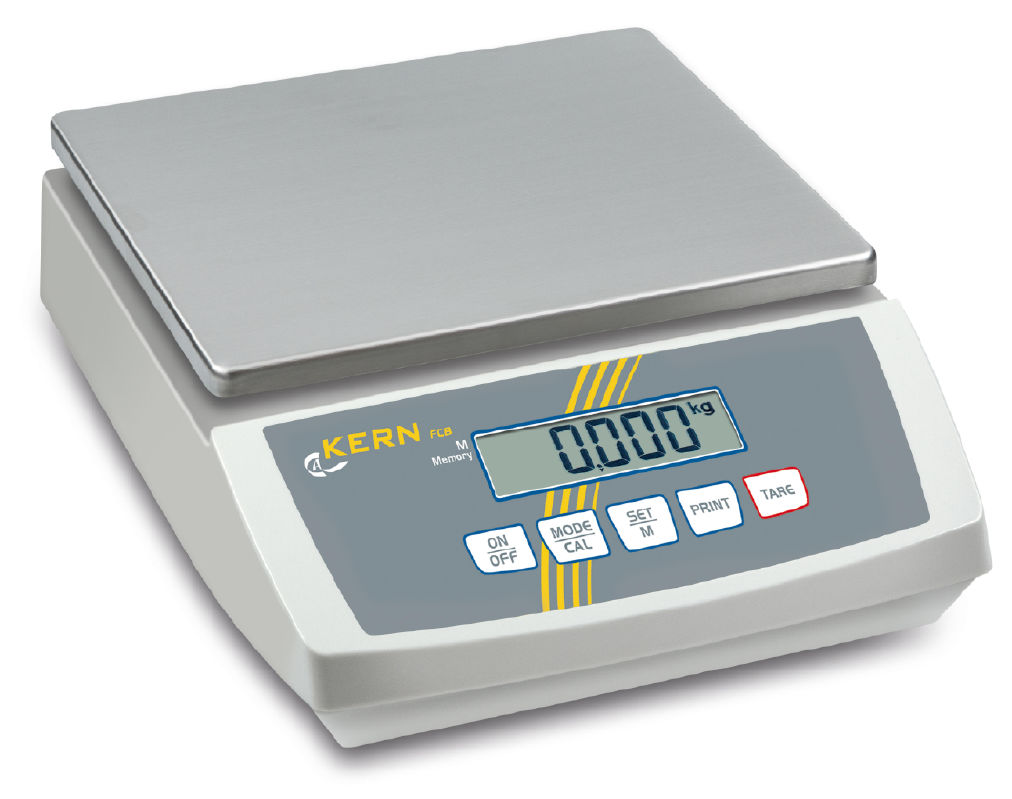
\includegraphics[scale=0.2]{Pictures/scale.jpg}
    \end{figure}
  }
  %%
  \uncover<1,3>{
  \begin{itemize}
    \item Center of mass
  \end{itemize}
  }
  \only<3>{
  \begin{figure}[H]
    \centering
    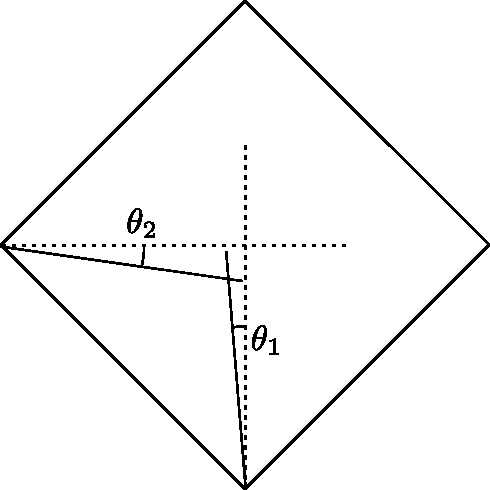
\includegraphics[scale=0.35]{Pictures/centerOfMassDiagram.pdf}
  \end{figure}
  }
  %%
  \uncover<1,4>{
  \begin{itemize}
    \item Friction and moment of inertia of the frame
  \end{itemize}
  }
  \only<4>{
    \begin{figure}[H]
    \centering
    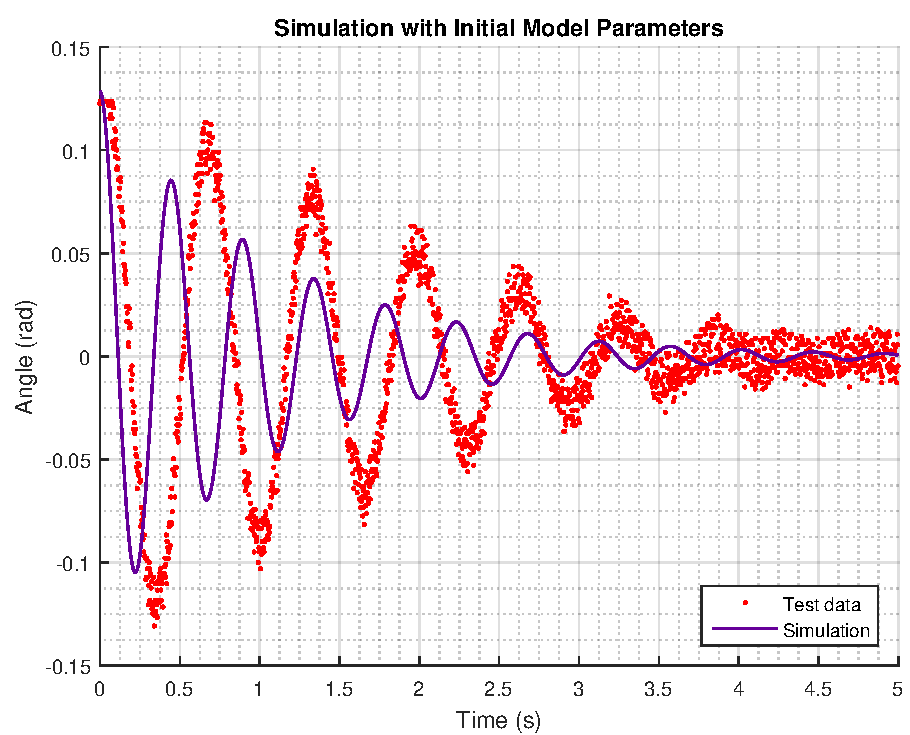
\includegraphics[scale=0.4]{Pictures/InitialModelParameterCompare.pdf}
  \end{figure}
  }
\end{frame}

%--------------------------------------------------------
\subsection{Parameter Estimation}

%- 3 -%
\begin{frame}{Parameter Estimation}{Optimization Problem}
  \begin{itemize}
    \item Optimization problem
  \end{itemize}  
  \begin{figure}[H]
      \centering
      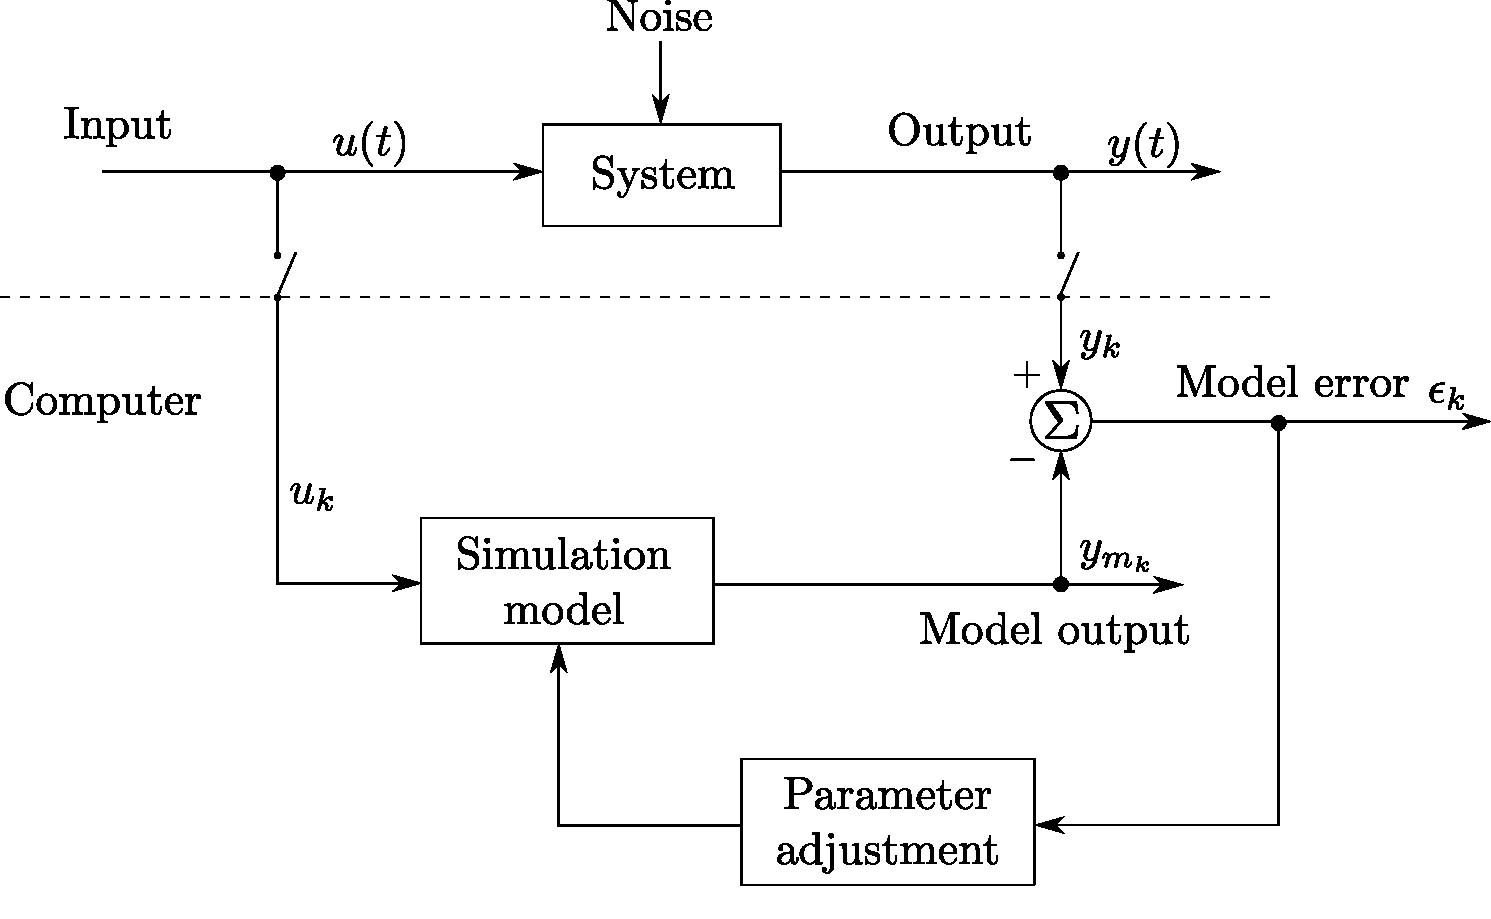
\includegraphics[scale=0.25]{Pictures/senstoolsModelOptimizationHM}
  \end{figure}\vspace{-12pt}
  \pause
  \begin{itemize}
    \item Cost function
  \end{itemize}
  \begin{displaymath}
    \si{C(\theta) = \frac{1}{2N}\sum_{k = 1}^{N} \left(y_{k} - y_{m_k}(\vec{\theta})\right)^2 }
  \end{displaymath}
\end{frame}

%- 4 -%
\begin{frame}{Parameter Estimation}{Steepest Descent (1)}
  \begin{figure}[H]
    \centering
    % (Must be redone)
    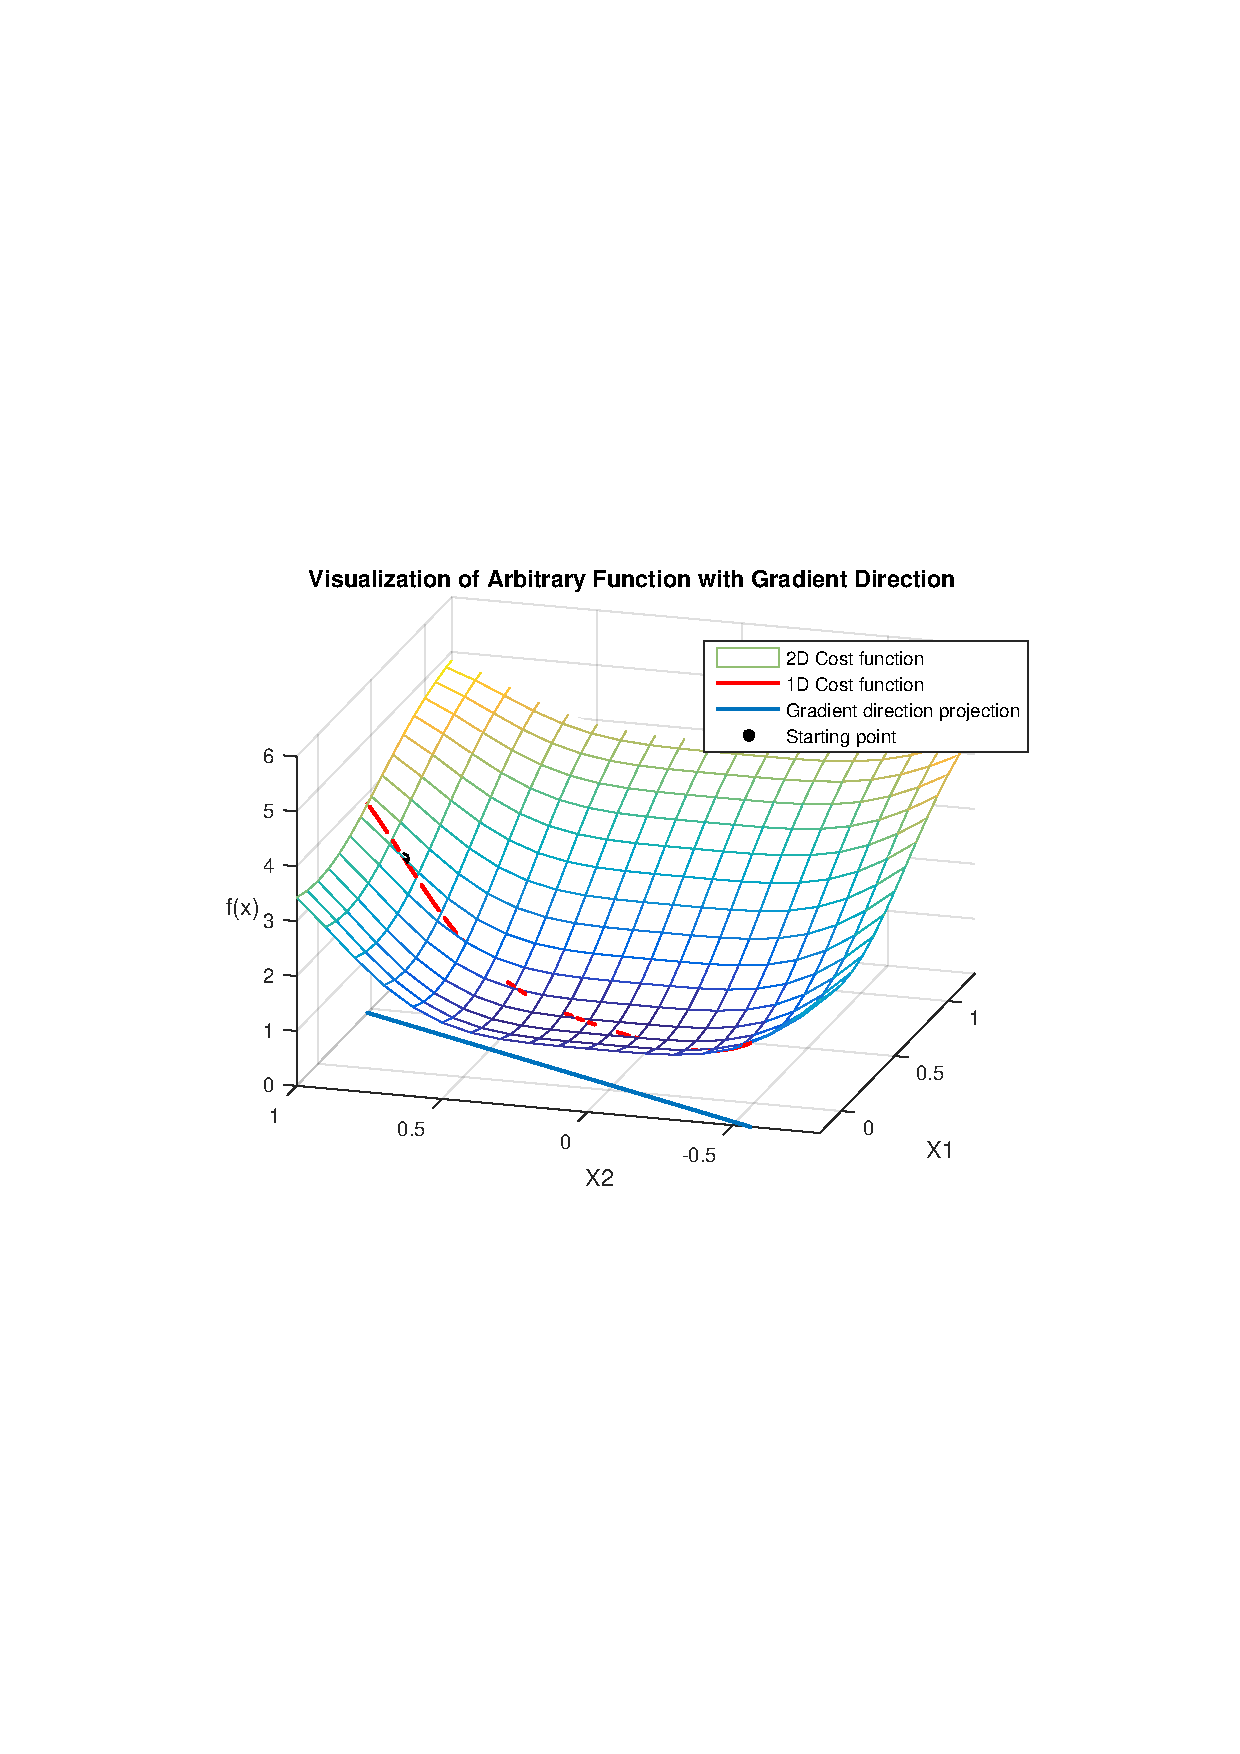
\includegraphics[scale=0.28]{Pictures/gradientDIrection2D4}
  \end{figure}
\end{frame}

\begin{frame}{Parameter Estimation}{Steepest Descent (2)}
  \begin{figure}[H]
    \centering
    % Plot of the 1D cost function along the gradient direction
    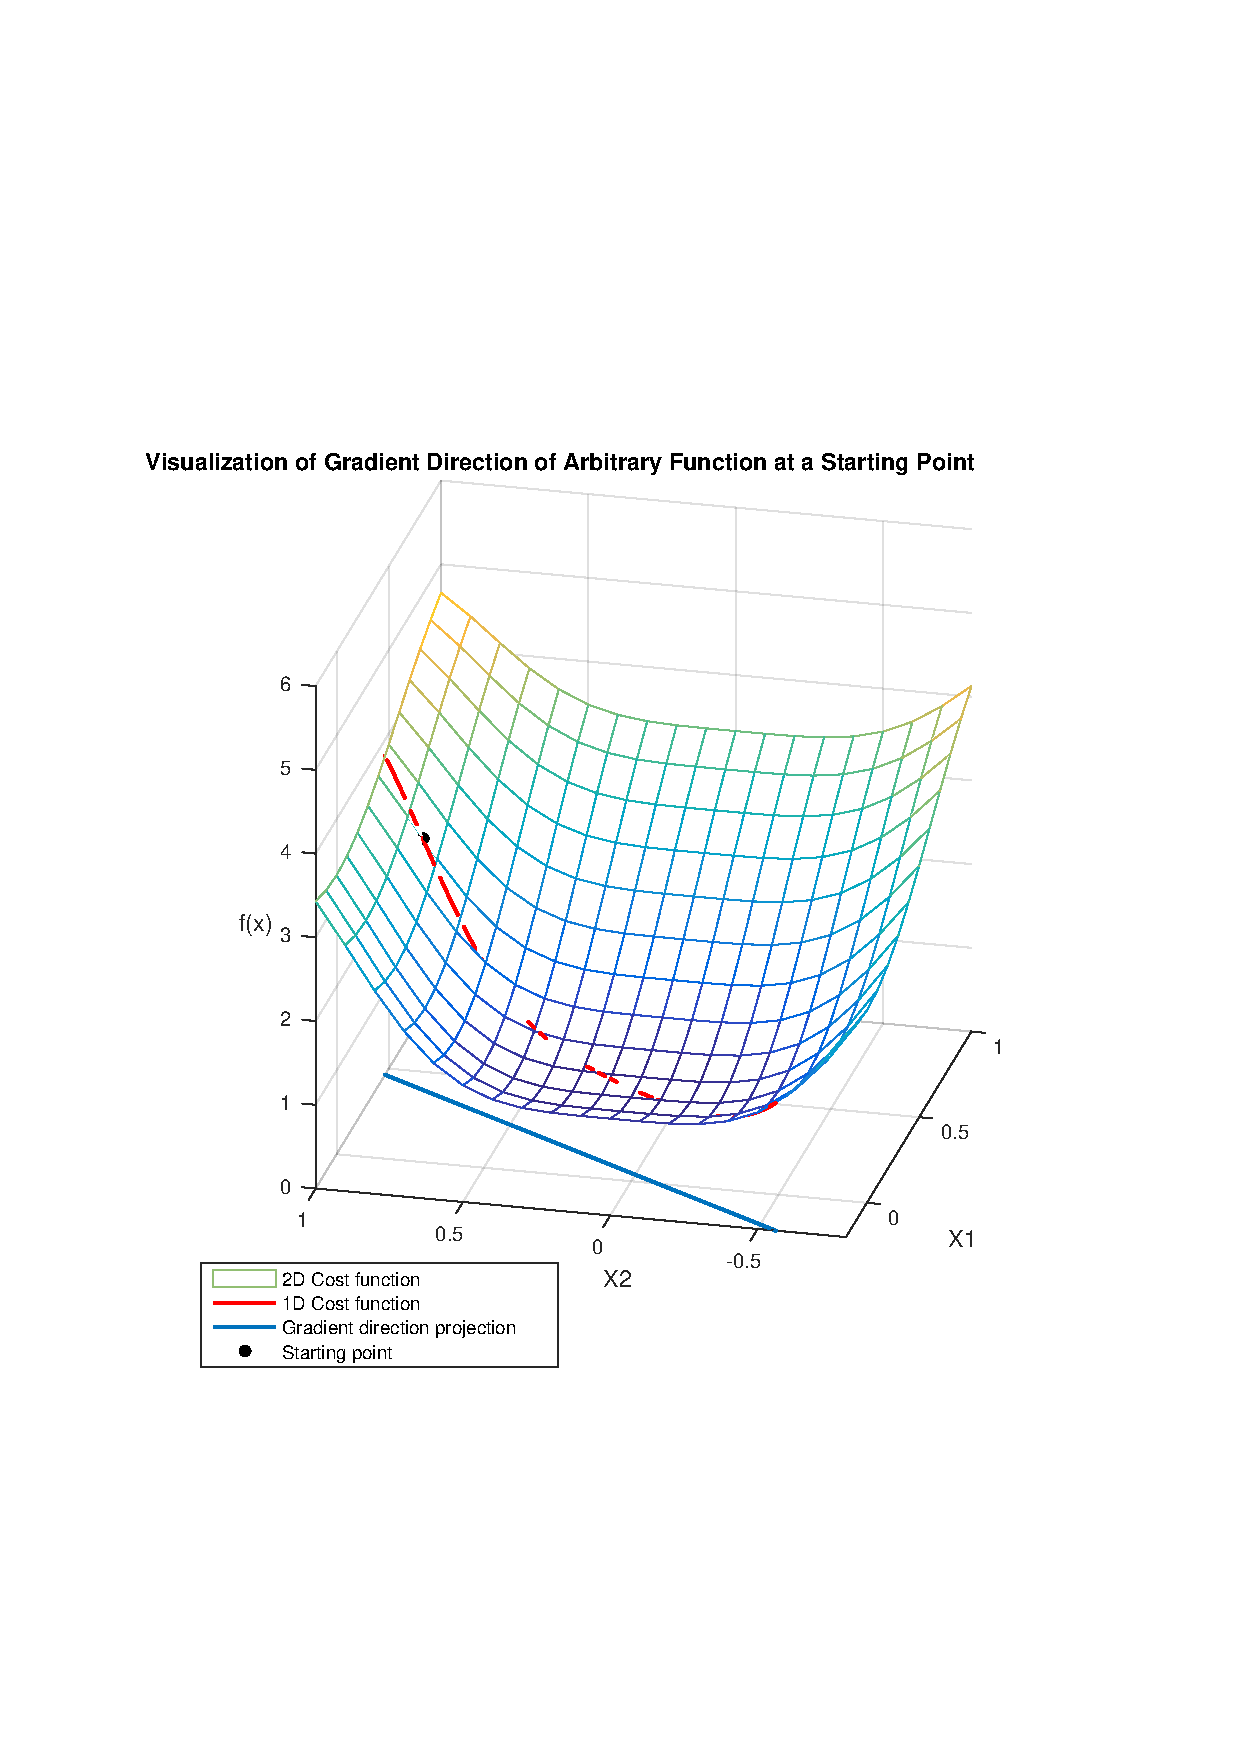
\includegraphics[scale=0.33]{Pictures/gradientDIrection1D3}
  \end{figure}
\end{frame}

%- 5 -%
\begin{frame}{Parameter Estimation}{Fibonacci Line Search}
  \begin{minipage}{\linewidth}
    \begin{minipage}{0.40\linewidth}
      \only<1>{
      \begin{figure}[H]
        \centering
        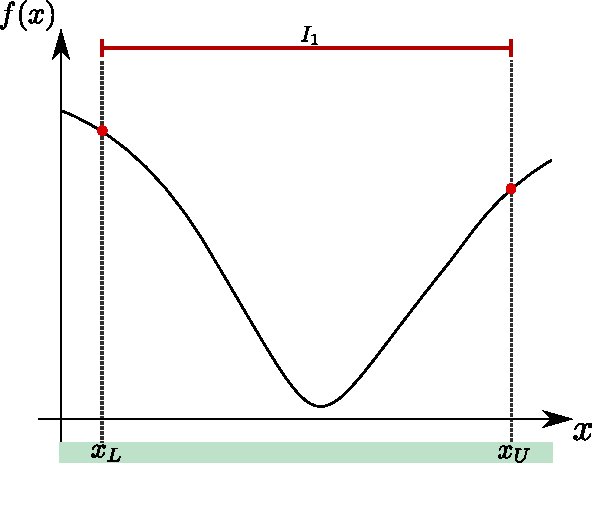
\includegraphics[scale=0.40]{Pictures/fibonacciIntervalSystem0}
      \end{figure}
      }
      \only<2>{
      \begin{figure}[H]
        \centering
        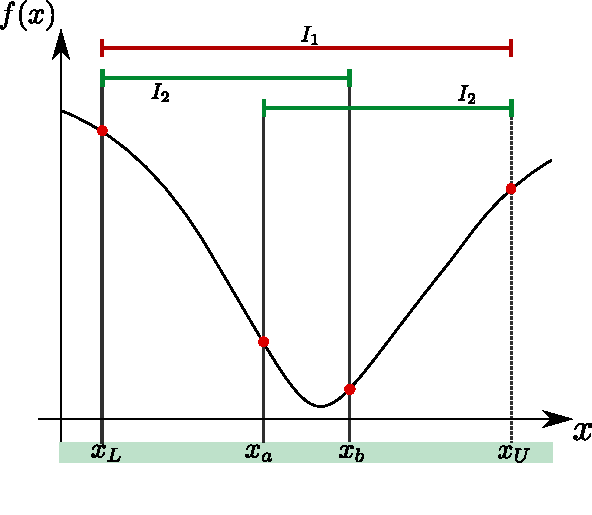
\includegraphics[scale=0.40]{Pictures/fibonacciIntervalSystem1}
      \end{figure}
      }
      \only<3>{
      \begin{figure}[H]
        \centering
        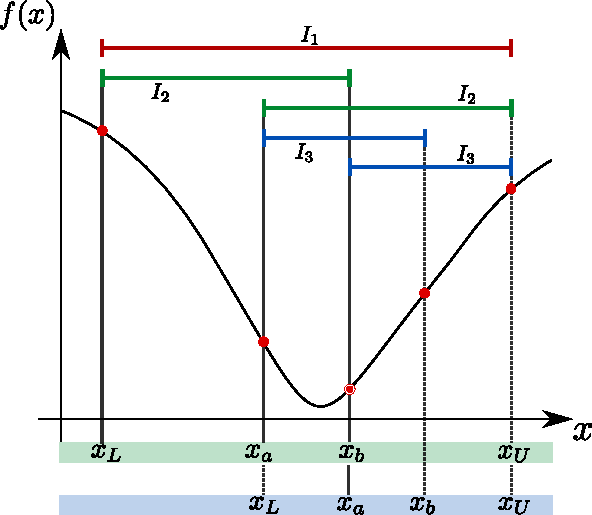
\includegraphics[scale=0.40]{Pictures/fibonacciIntervalSystem2}
      \end{figure}
      }
      \only<4->{
      \begin{figure}[H]
        \centering
        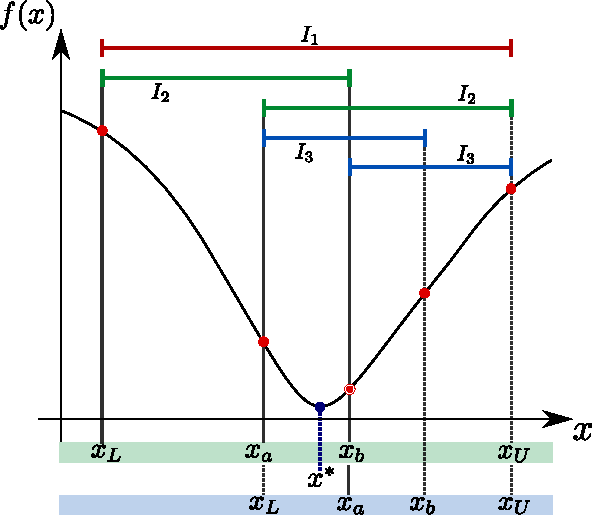
\includegraphics[scale=0.40]{Pictures/fibonacciIntervalSystem3}
      \end{figure}
      }
    \end{minipage}
    % \hspace{0.05\linewidth}
    \begin{minipage}{0.45\linewidth}
      \pause[5]
      % \only<5->{
        \begin{itemize}
          \item Initial relations
        \end{itemize}
        \begin{displaymath}
          \si{I_k = I_{k+1} + I_{k+2}, for\ all\ k=1,2,\dots,n-1}
        \end{displaymath}
        \begin{displaymath}
          \si{I_n = I_{n+1},\ assuming\ I_{n+2}=0}
        \end{displaymath}
      % }
      \vspace{-12pt}
      %%
      \pause[6]
      % \only<6>{  
        \begin{itemize}
          \item Successive relations
        \end{itemize}
        \begin{displaymath}
          \si{I_{n+1}}      =  \phantom{\si{\ I_{n+1}  + I_{n+2}         =}}\si{ 1 I_n  = F_0 I_n}
        \end{displaymath}
        \begin{displaymath}
          \si{I_{n}}\phantom{_{+1}}      =  \si{ I_{n+1}  + I_{n+2} }                    =  \si{ 1 I_n  = F_1 I_n }
        \end{displaymath}
        \begin{displaymath}
          \si{I_{n-1}}      =  \si{ I_{n} }\phantom{_{+1}} + \si{ I_{n+1} } =  \si{ 2 I_n  = F_2 I_n }
        \end{displaymath}
        \begin{displaymath}
          \vdots
          \phantom{I_{n-4}+I_{n-5}+I{4242}}
        \end{displaymath}
        \begin{displaymath}
          \si{I_{k}}\phantom{_{4}}   =  \si{ I_{k+1} + I_{k+2} = F_{n-k+1} I_n }
        \end{displaymath}
        \begin{displaymath}
          \vdots                         
          \phantom{I_{n-4}+I_{n-5}+I{4242}}
        \end{displaymath}
        \begin{displaymath}
          \si{I_{1}}\phantom{_{4}}      =  \si{ I_{2}  + I_{3} }\si{= F_n I_n }\phantom{_{k-1k+2k+3}} 
        \end{displaymath}
      % }
    \end{minipage}
  \end{minipage}
\end{frame}


%----------------------------------------------------------------
\begin{frame}{Parameter Estimation}{Forward-Backward Method}
  \begin{itemize}
    \item Goal: find an initial bracket
    \item Principle: high-low-high geometry
  \end{itemize}
  \begin{figure}[H]
    \centering
    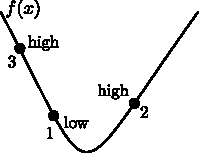
\includegraphics[scale=1.5]{Pictures/forward-backward.pdf}
  \end{figure}
\end{frame}

% \begin{frame}{Parameter Estimation}{Implementation (1)}
%   \begin{minipage}{\linewidth}\centering
%     \begin{minipage}{0.35\linewidth}
%       \begin{figure}[H]
%         \centering
%         %\transduration<0-19>{0}
%         %\multiinclude[<+->][format=png, graphics={width=\textwidth}]{Pictures/cost}
%         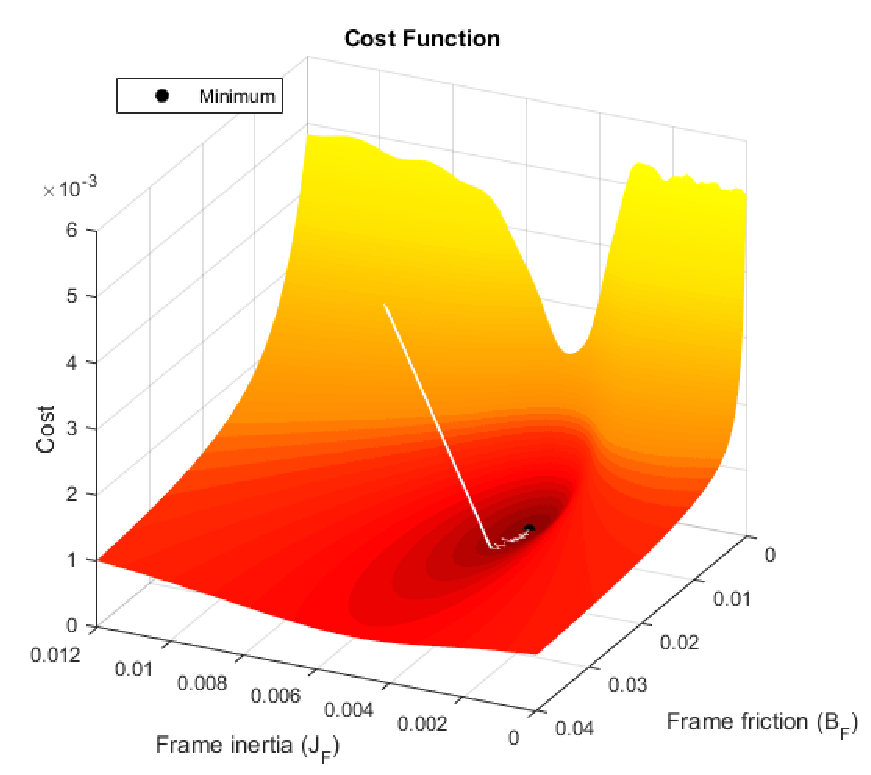
\includegraphics[scale=0.35]{Pictures/costFunctionMinimized.pdf}       
%       \end{figure}
%     \end{minipage}
%     \hspace{0.15\linewidth}
%     \begin{minipage}{0.45\linewidth}
%       \begin{figure}[H]
%         \centering
%         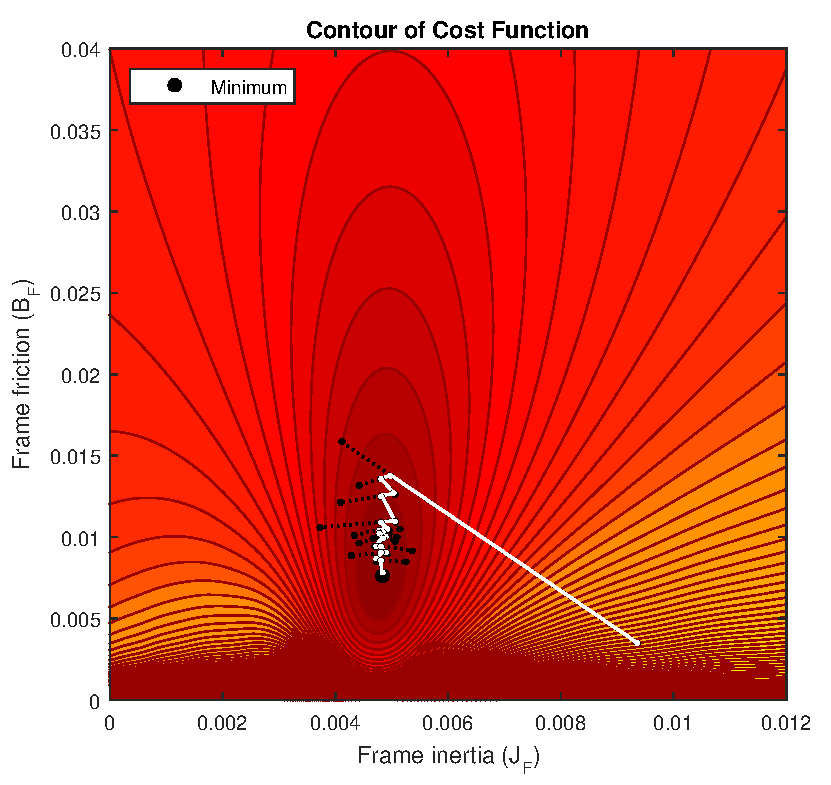
\includegraphics[scale=0.35]{Pictures/costFunctionMinimizedContour.pdf}
%       \end{figure}
%     \end{minipage}
%   \end{minipage}
%   Animated pictures would be better...
% \end{frame}

\begin{frame}{Parameter Estimation}{Implementation (1)}
  \begin{figure}[H]
    \centering
    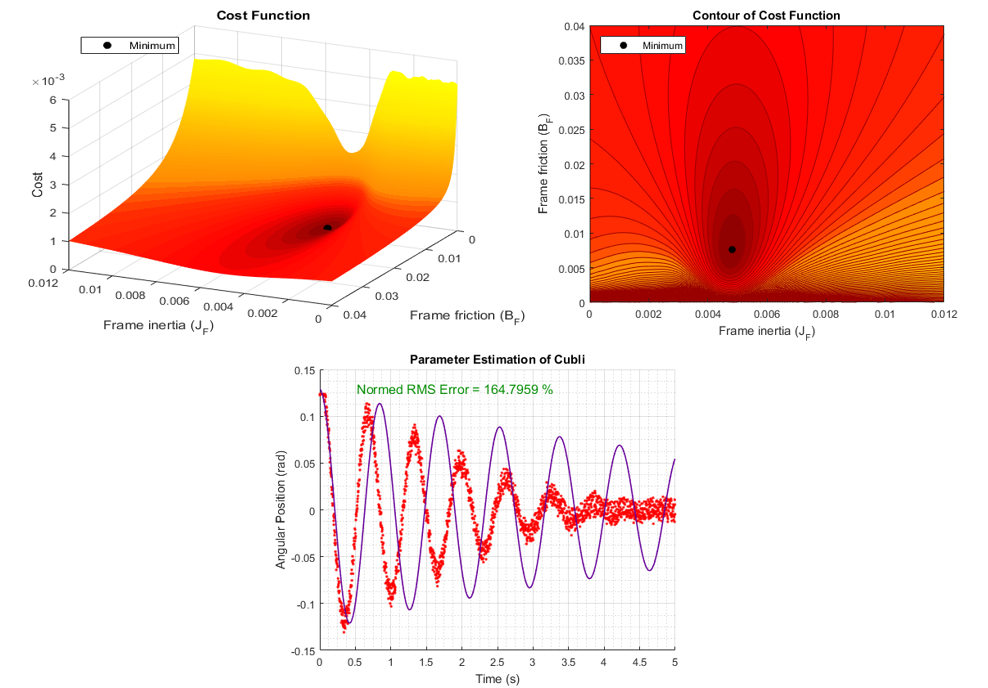
\includegraphics[width=\textwidth]{Pictures/optJoinedFit/cost-0.png}
  \end{figure}
\end{frame}

\begin{frame}{Parameter Estimation}{Implementation (1)}
  \transduration<1-19>{0.75}
  \multiinclude[format=png, graphics={width=\textwidth}]{Pictures/optJoinedFit/cost}
  %\animategraphics[autoplay,loop,width=\linewidth]{1}{Pictures/cost-}{0}{19}
\end{frame}

\begin{frame}{Parameter Estimation}{Implementation (2)}
  \begin{minipage}{\linewidth}\centering
    \begin{minipage}{0.45\linewidth}
      \only<1->{
      \begin{figure}[H]
        \centering
        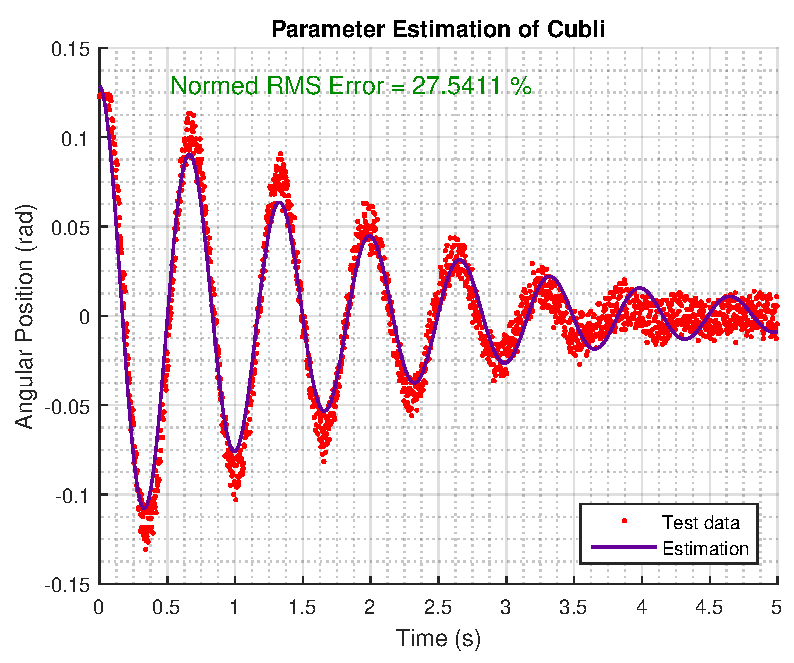
\includegraphics[scale=0.35]{Pictures/resultOfGradientWithFibonacciAndForwardBackward}
      \end{figure}
        \begin{table}[H]\centering
          \begin{tabular}{
          |c
          |S[table-figures-exponent=1,table-number-alignment=left, table-figures-integer=1]%@{\,}
          |s[table-unit-alignment = left,table-column-width=52pt]|}
            % \hline
              % \textbf{Parameter}  & \multicolumn{1}{c|}{\textbf{Value}} & \multicolumn{1}{c|}{\textbf{Unit}}\\
            \hline%------------------------------------------------------------------
              \si{J_F}            & 4.8e-3 & \kilo\gram\meter\squared         \\%& -\\
            % \hline%------------------------------------------------------------------
              \si{B_F}            & 7.8e-3 & \newton\metre\second\per\radian            \\%& -\\
            \hline%------------------------------------------------------------------
          \end{tabular}
        \end{table}
      }
    \end{minipage}
    \hspace{0.05\linewidth}
    \begin{minipage}{0.45\linewidth}
      % \only<2->{
      \pause[2]
        \begin{figure}[H]
          \centering
          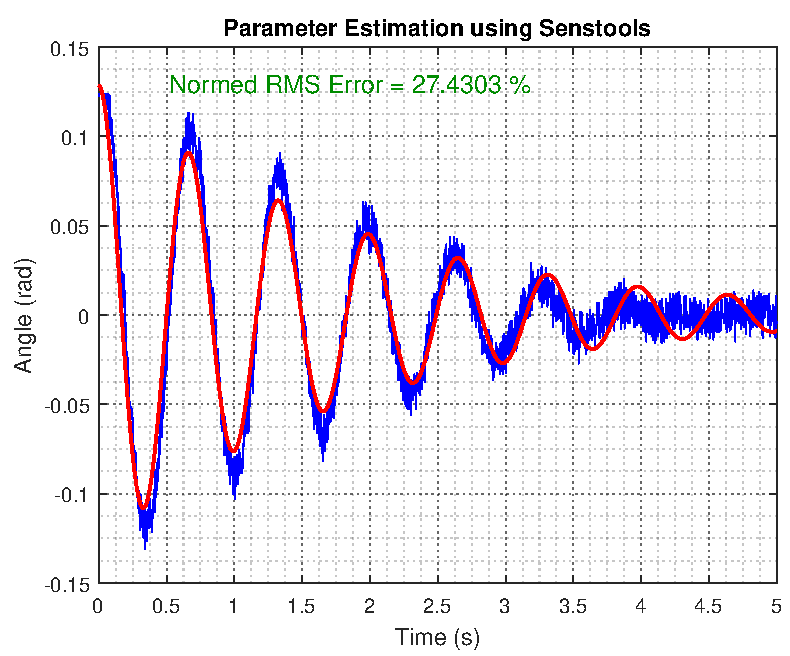
\includegraphics[scale=0.35]{Pictures/SenseToolParameterEstimation}
        \end{figure}
        \begin{table}[H]\centering
          \begin{tabular}{
          |c
          |S[table-figures-exponent=1,table-number-alignment=left, table-figures-integer=1]%@{\,}
          |s[table-unit-alignment = left,table-column-width=52pt]|}
            % \hline
              % \textbf{Parameter}  & \multicolumn{1}{c|}{\textbf{Value}} & \multicolumn{1}{c|}{\textbf{Unit}}\\
            \hline%------------------------------------------------------------------
              \si{J_F}            & 4.8e-3 & \kilo\gram\meter\squared             \\%& -\\
            % \hline%------------------------------------------------------------------
              \si{B_F}            & 7.7e-3 & \newton\metre\second\per\radian            \\%& -\\
            \hline%------------------------------------------------------------------
          \end{tabular}
        \end{table}
      % }
    \end{minipage}
  \end{minipage}
\end{frame}

%------------------------------------------------------------
\subsection{Model Parameters (rev'd)}

\begin{frame}{Model Parameters}{Final Parameters}
  \begin{table}[H]\centering
  \begin{tabular}{
  |c
  |S[
    table-figures-exponent=2,
    % table-column-width=60pt
    % table-figures-integer=2,
    % table-number-alignment=right
    ]
  |s[table-unit-alignment = left]|
  }
    \hline
      \textbf{Parameter}  & \multicolumn{1}{c|}{\textbf{Value}} & \multicolumn{1}{c|}{\textbf{Unit}}\\
    \hline%------------------------------------------------------------------
      \si{m_W}            & 0.222                               & \kilo\gram\\
    % \hline%------------------------------------------------------------------
      \si{l_W}            & 0.093                               & \metre\\
    % \hline%------------------------------------------------------------------
      \si{J_W}            & 0.601e-3                            & \kilo\gram\meter\squared\\
    % \hline%------------------------------------------------------------------
      \si{B_W}            & 17.03e-6                            & \newton\metre\second\per\radian\\
    % \hline%------------------------------------------------------------------
      \si{m_F}            & 0.548                               & \kilo\gram\\
    % \hline%------------------------------------------------------------------
      \si{l_F}            & 0.08498                             & \metre\\
    % \hline%------------------------------------------------------------------
      \si{J_F}            & 4.8e-3                              & \kilo\gram\meter\squared \\
    % \hline%------------------------------------------------------------------
      \si{B_F}            & 7.7e-3                              & \newton\metre\second\per\radian\\
    \hline%------------------------------------------------------------------
  \end{tabular}
  \end{table}
\end{frame}

\section{Model Testing}
\begin{frame}{Model Testing}{Linearization of the Model}
  \begin{minipage}{\linewidth}\centering
    \begin{minipage}{0.45\linewidth}
      \begin{figure}[H]
        \centering
        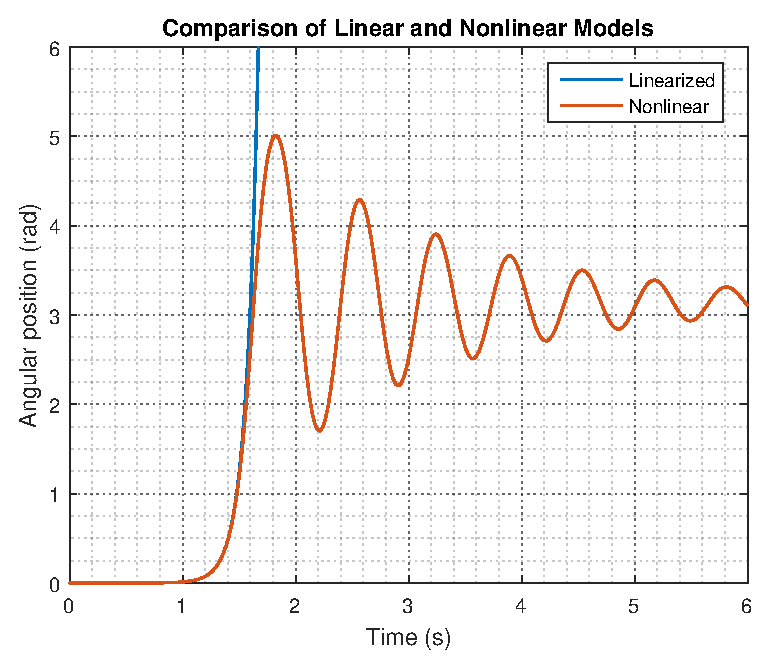
\includegraphics[scale=0.33]{Pictures/LinearizedVSNonlinear}
      \end{figure}
    \end{minipage}
    % \hspace{0.05\linewidth}
    \begin{minipage}{0.45\linewidth}
      \begin{figure}[H]
        \centering
        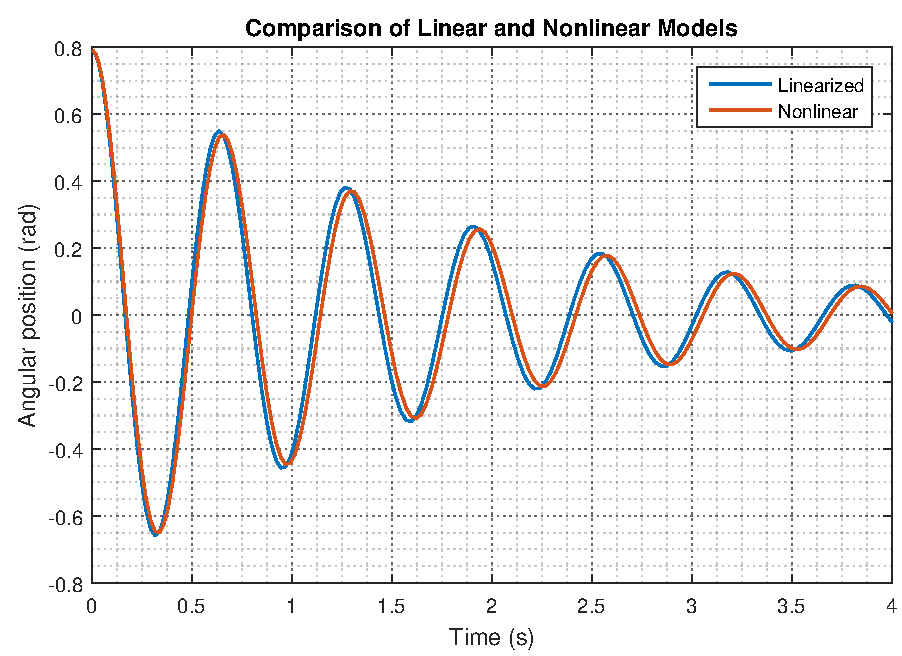
\includegraphics[scale=0.33]{Pictures/LinearizedVSNonlinear_0}
      \end{figure}
    \end{minipage}
  \end{minipage}
\end{frame}

\begin{frame}{Model Testing}{Comparison with Real System}
  \begin{minipage}{\linewidth}\centering
    \begin{minipage}{0.45\linewidth}
      \begin{figure}[H]
        \centering
        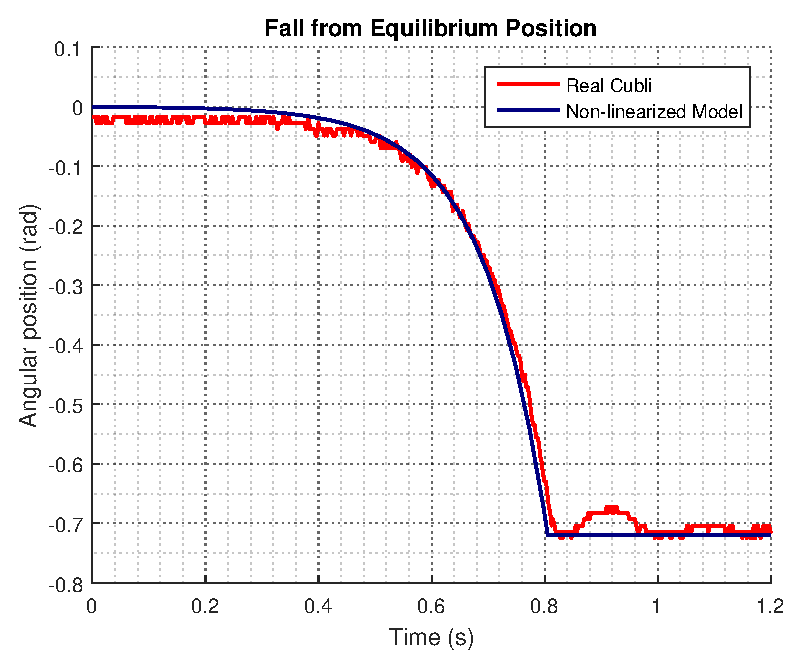
\includegraphics[scale=0.33]{Pictures/FallTestComparison}
      \end{figure}
    \end{minipage}
    \hspace{0.03\linewidth}
    \begin{minipage}{0.45\linewidth}
      \begin{figure}[H]
        \centering
        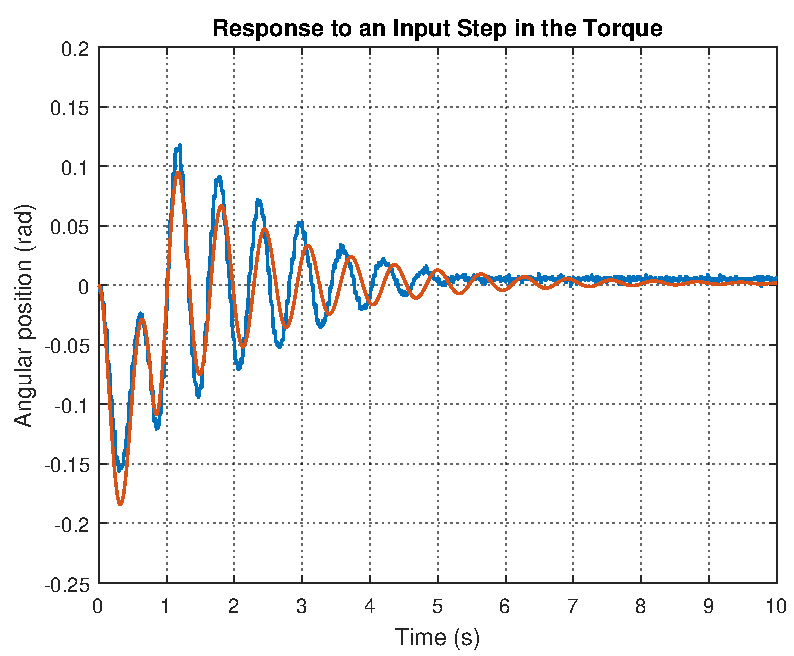
\includegraphics[scale=0.33]{Pictures/StepTest}
      \end{figure}
    \end{minipage}
  \end{minipage}
\end{frame}
	%%%%%%%%%%%%%%%%%%%%%%%%%%%%%%%%%% NAME %%%%%%%%%%%%%%%%%%%%%%%%%%%%%

%%%%%%%%%%%%%%%%%
\section{Stability Analysis}

\subsection{Root Locus}
\begin{frame}{Stability Analysis}{Root Locus}
\begin{minipage}{\linewidth}
	\begin{minipage}{0.45\linewidth}
		\begin{figure}
			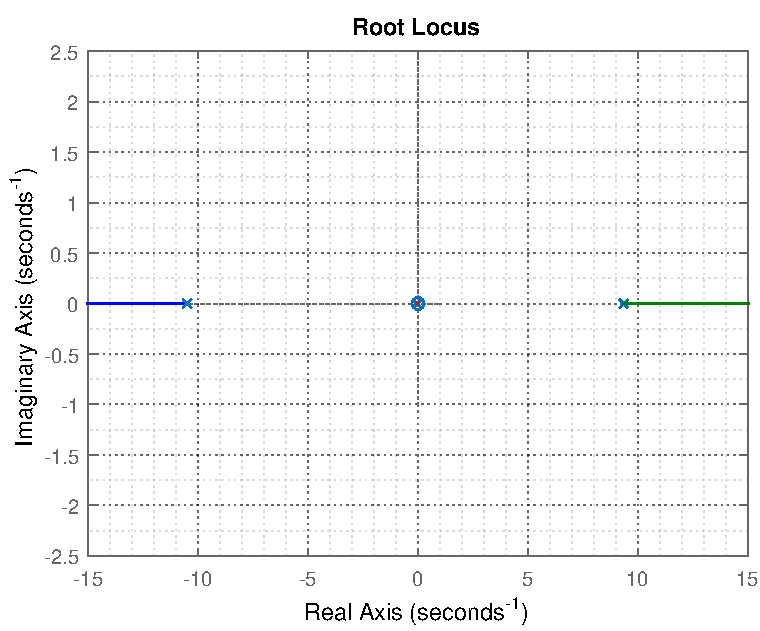
\includegraphics[scale=.42]{Pictures/rlocusCubli}
			\centering
		\end{figure}
	\end{minipage}
	\hspace{0.1\linewidth}
	\begin{minipage}{0.45\linewidth}
		\begin{figure}[H]
			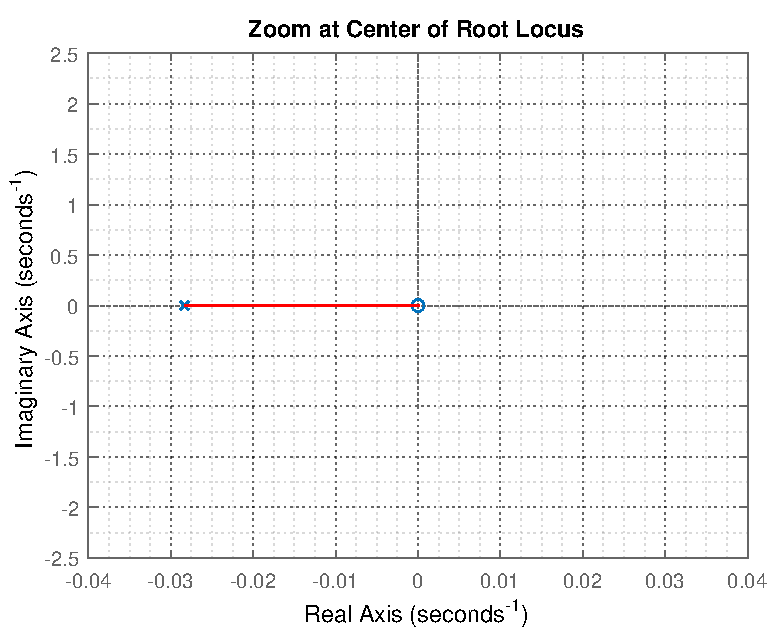
\includegraphics[scale=.35]{Pictures/rlocusCubliZoom}
			\centering
		\end{figure}
	\end{minipage}
\end{minipage}
\end{frame}

\subsection{Nyquist Plot}
\begin{frame}{Stability Analysis}{Nyquist Plot}
\begin{figure}
		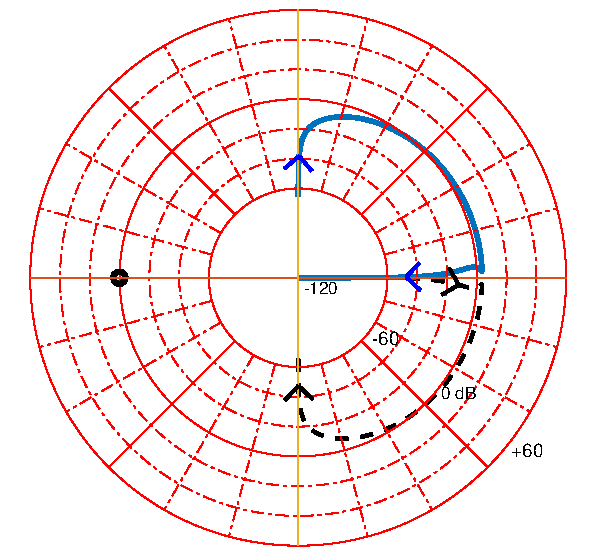
\includegraphics[scale=.56]{Pictures/nyquistCubli}
		\centering
\end{figure}
	
\end{frame}
%%%%%%%%%%%%%%%%%

%%%%%%%%%%%%%%%%%
\section{Classical Controller Design}

\subsection{Root Locus}
\begin{frame}{Classical Controller Design}{}	
\begin{figure}
	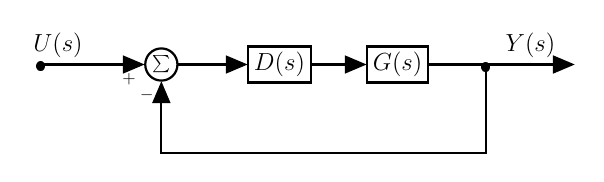
\begin{tikzpicture}[ auto,
thick,                         %<--setting line style
node distance=1.5cm,             %<--setting default node distance
scale=0.75,                     %<--|these two scale the whole thing
every node/.style={scale=0.62}, %<  |(always change both)
>=triangle 45 ]

%-- Blocks creation --%
\draw
% DIRECT TERM %
node[shape=coordinate][](input1) at (0,0){}
node[shape=coordinate][](feed) at (0.5,0){}
node(sum1) at (2,0) [sum] {$\sum$}
node(controller) at (4,0) [block]{\Large $D(s)$}
node(plant) at (6,0) [block]{\Large $G(s)$}
node[shape=coordinate][](DummyNode) at (5,-1.5){}
node[shape=coordinate][](FeedbackNode) at (7.5,0){}
;

%-- Block linking --%
% INPUT %
\draw[-](input1)        -- node{\Large $U(s)$}(feed);
\draw[->](feed)  -- (sum1);

% OUTPUT %
\draw[-](plant)  -- (FeedbackNode);
\draw[->](FeedbackNode)       -- node {\Large $Y(s)$} (9,0);

% DIRECT TERM %
\draw[->] (sum1)            -- (controller);
\draw[->] (controller)       -- (plant);

% FEEDBACKS %
\draw[-] (FeedbackNode)  |- (DummyNode);
\draw[->] (DummyNode)  -| (sum1);

%-- Nodes --%
\draw%--------------------------------------------------------------
node at (input1)            [shift={(-0.04, -0.05 )}] {\Large \textbullet}
node at (FeedbackNode)      [shift={(0, -0.07 )}] {\Large \textbullet}
;
%-- Summation signs --%
\draw%--------------------------------------------------------------
node at (sum1) [right = -6.6mm, below = .6mm] {$+$}
node at (sum1) [right = -3mm, below = 3.9mm]  {$-$}
;

\end{tikzpicture} 
\end{figure}
\end{frame}

\subsection{Root Locus}
\begin{frame}{Classical Controller Design}{}
	
	\begin{figure}
		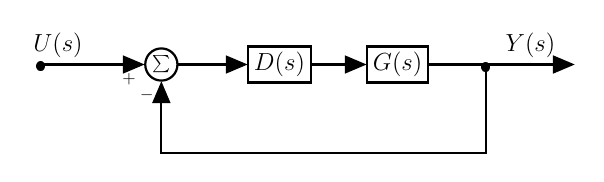
\begin{tikzpicture}[ auto,
thick,                         %<--setting line style
node distance=1.5cm,             %<--setting default node distance
scale=0.75,                     %<--|these two scale the whole thing
every node/.style={scale=0.62}, %<  |(always change both)
>=triangle 45 ]

%-- Blocks creation --%
\draw
% DIRECT TERM %
node[shape=coordinate][](input1) at (0,0){}
node[shape=coordinate][](feed) at (0.5,0){}
node(sum1) at (2,0) [sum] {$\sum$}
node(controller) at (4,0) [block]{\Large $D(s)$}
node(plant) at (6,0) [block]{\Large $G(s)$}
node[shape=coordinate][](DummyNode) at (5,-1.5){}
node[shape=coordinate][](FeedbackNode) at (7.5,0){}
;

%-- Block linking --%
% INPUT %
\draw[-](input1)        -- node{\Large $U(s)$}(feed);
\draw[->](feed)  -- (sum1);

% OUTPUT %
\draw[-](plant)  -- (FeedbackNode);
\draw[->](FeedbackNode)       -- node {\Large $Y(s)$} (9,0);

% DIRECT TERM %
\draw[->] (sum1)            -- (controller);
\draw[->] (controller)       -- (plant);

% FEEDBACKS %
\draw[-] (FeedbackNode)  |- (DummyNode);
\draw[->] (DummyNode)  -| (sum1);

%-- Nodes --%
\draw%--------------------------------------------------------------
node at (input1)            [shift={(-0.04, -0.05 )}] {\Large \textbullet}
node at (FeedbackNode)      [shift={(0, -0.07 )}] {\Large \textbullet}
;
%-- Summation signs --%
\draw%--------------------------------------------------------------
node at (sum1) [right = -6.6mm, below = .6mm] {$+$}
node at (sum1) [right = -3mm, below = 3.9mm]  {$-$}
;

\end{tikzpicture} 
	\end{figure}
\end{frame}

\subsection{Final Controller}
\begin{frame}{Root Locus Designed Controller}{Final Root Locus}
\begin{figure}
	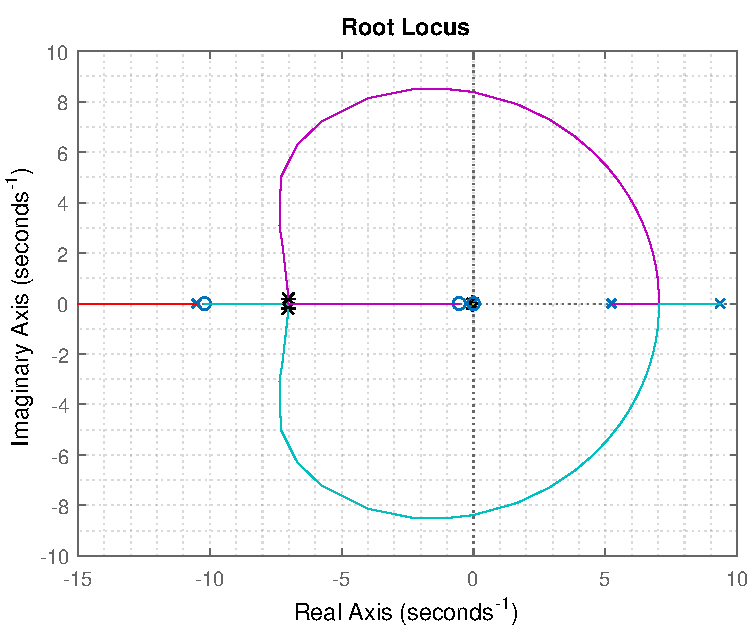
\includegraphics[scale=.56]{Pictures/RLController}
	\centering
\end{figure}		
\end{frame}

\begin{frame}{Root Locus Designed Controller}{}
	
	\begin{figure}
		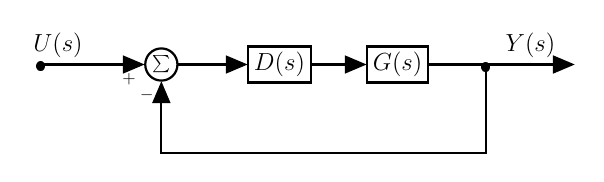
\begin{tikzpicture}[ auto,
thick,                         %<--setting line style
node distance=1.5cm,             %<--setting default node distance
scale=0.75,                     %<--|these two scale the whole thing
every node/.style={scale=0.62}, %<  |(always change both)
>=triangle 45 ]

%-- Blocks creation --%
\draw
% DIRECT TERM %
node[shape=coordinate][](input1) at (0,0){}
node[shape=coordinate][](feed) at (0.5,0){}
node(sum1) at (2,0) [sum] {$\sum$}
node(controller) at (4,0) [block]{\Large $D(s)$}
node(plant) at (6,0) [block]{\Large $G(s)$}
node[shape=coordinate][](DummyNode) at (5,-1.5){}
node[shape=coordinate][](FeedbackNode) at (7.5,0){}
;

%-- Block linking --%
% INPUT %
\draw[-](input1)        -- node{\Large $U(s)$}(feed);
\draw[->](feed)  -- (sum1);

% OUTPUT %
\draw[-](plant)  -- (FeedbackNode);
\draw[->](FeedbackNode)       -- node {\Large $Y(s)$} (9,0);

% DIRECT TERM %
\draw[->] (sum1)            -- (controller);
\draw[->] (controller)       -- (plant);

% FEEDBACKS %
\draw[-] (FeedbackNode)  |- (DummyNode);
\draw[->] (DummyNode)  -| (sum1);

%-- Nodes --%
\draw%--------------------------------------------------------------
node at (input1)            [shift={(-0.04, -0.05 )}] {\Large \textbullet}
node at (FeedbackNode)      [shift={(0, -0.07 )}] {\Large \textbullet}
;
%-- Summation signs --%
\draw%--------------------------------------------------------------
node at (sum1) [right = -6.6mm, below = .6mm] {$+$}
node at (sum1) [right = -3mm, below = 3.9mm]  {$-$}
;

\end{tikzpicture} 
	\end{figure}
	
\end{frame}

\begin{frame}{Root Locus Designed Controller}{}
	
	\begin{figure}
		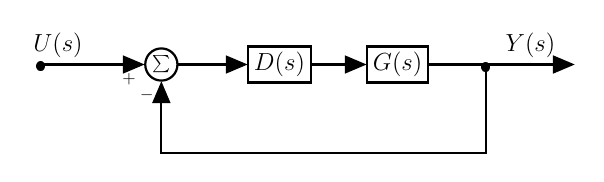
\begin{tikzpicture}[ auto,
thick,                         %<--setting line style
node distance=1.5cm,             %<--setting default node distance
scale=0.75,                     %<--|these two scale the whole thing
every node/.style={scale=0.62}, %<  |(always change both)
>=triangle 45 ]

%-- Blocks creation --%
\draw
% DIRECT TERM %
node[shape=coordinate][](input1) at (0,0){}
node[shape=coordinate][](feed) at (0.5,0){}
node(sum1) at (2,0) [sum] {$\sum$}
node(controller) at (4,0) [block]{\Large $D(s)$}
node(plant) at (6,0) [block]{\Large $G(s)$}
node[shape=coordinate][](DummyNode) at (5,-1.5){}
node[shape=coordinate][](FeedbackNode) at (7.5,0){}
;

%-- Block linking --%
% INPUT %
\draw[-](input1)        -- node{\Large $U(s)$}(feed);
\draw[->](feed)  -- (sum1);

% OUTPUT %
\draw[-](plant)  -- (FeedbackNode);
\draw[->](FeedbackNode)       -- node {\Large $Y(s)$} (9,0);

% DIRECT TERM %
\draw[->] (sum1)            -- (controller);
\draw[->] (controller)       -- (plant);

% FEEDBACKS %
\draw[-] (FeedbackNode)  |- (DummyNode);
\draw[->] (DummyNode)  -| (sum1);

%-- Nodes --%
\draw%--------------------------------------------------------------
node at (input1)            [shift={(-0.04, -0.05 )}] {\Large \textbullet}
node at (FeedbackNode)      [shift={(0, -0.07 )}] {\Large \textbullet}
;
%-- Summation signs --%
\draw%--------------------------------------------------------------
node at (sum1) [right = -6.6mm, below = .6mm] {$+$}
node at (sum1) [right = -3mm, below = 3.9mm]  {$-$}
;

\end{tikzpicture} 
	\end{figure}
	
\end{frame}
%%%%%%%%%%%%%%%%%

	%%%%%%%%%%%%%%%%%%%%%%%%%%%%%%%%%%% Niels %%%%%%%%%%%%%%%%%%%%%%%%%%%%%
%%%%%%%%%%%%%%%%%
\section{State Space}

%---------------------------------------------------------------------------------
\subsection{Motivation}%----------------------------------------------------------
%---------------------------------------------------------------------------------

\begin{frame}{State Space}{Motivation}	
  \begin{itemize}
  	\item Angular velocity of the wheel using root locus design
  \end{itemize}
  \vspace{.5cm}
  \begin{minipage}{\linewidth}
  	\begin{minipage}{0.4\linewidth}
  		\begin{figure}
  			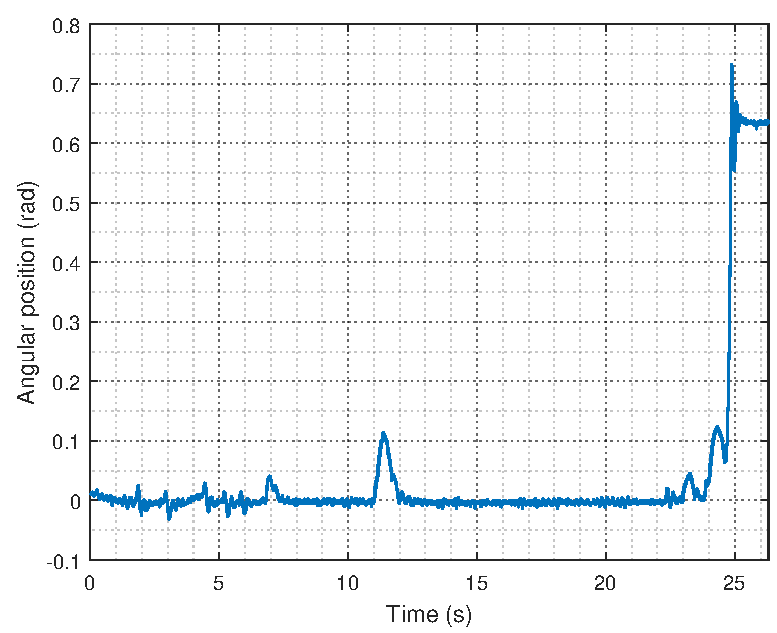
\includegraphics[scale=.35]{Pictures/positionRLTest}
  			\centering
  		\end{figure}
  	\end{minipage}
  	\hspace{0.1\linewidth}
  	\begin{minipage}{0.45\linewidth}
  		\begin{figure}[H]
  			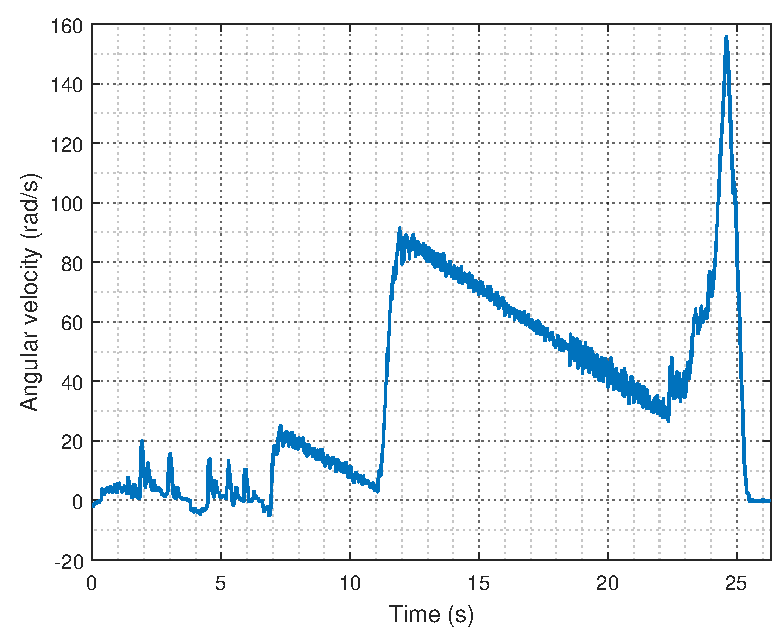
\includegraphics[scale=.35]{Pictures/wheelRLTest}
  			\centering
  		\end{figure}
  	\end{minipage}
  \end{minipage}
\end{frame}

\begin{frame}{State Space}{Motivation}
  \begin{itemize}
    \item Control of velocity for improved performance
    \item Classical cascade control is not feasible
  \end{itemize}
  \vspace{.2cm}
  \begin{figure}[H]
    \centering
      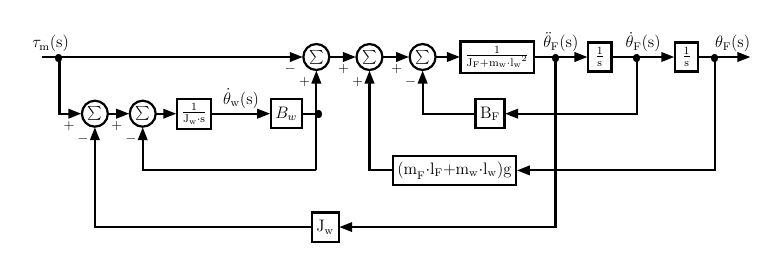
\begin{tikzpicture}[ auto,
                       thick,                         %<--setting line style
                       node distance=1.5cm,             %<--setting default node distance
                       scale=0.45,                     %<--|these two scale the whole thing
                       every node/.style={scale=0.50}, %<  |(always change both)
                       >/.tip={Triangle[angle=40:5pt]}
                       ]

    %-- Blocks creation --%
    \draw
      % DIRECT TERM %
      node[shape=coordinate][](input1) at (0,0){}
      node[shape=coordinate][](feedForward) at (0.5,0){}
      node(sum1) at (7.75,0) [sum] {\si{\sum}}
      node(sum2) at (9.25,0) [sum]{\si{\sum}}
      node(sum3) at (10.75,0) [sum]{\si{\sum}}

      node(torque2rotacc1) at (12.85,0) [block]{\large \si{\frac{1}{J_F + m_w \cdot {l_w}^{2}}}}

      node(integration1) at (15.75,0) [block] {\large \si{\frac{1}{s}}}
      node(integration2) at (18.2,0) [block] {\large \si{\frac{1}{s}}}

      node[shape=coordinate][](output) at (19,0){}
      node[shape=coordinate][](veloFeedbackNode) at (16.8,0){}
      node[shape=coordinate][](accFeedbackNode) at (14.5,0){}
    ;
    \draw
      % REACTION WHEEL EQUATIONS %  
      node(sum4) at (1.5,-1.6) [sum]{\si{\sum}}
      node(sum5) at (2.85,-1.6) [sum]{\si{\sum}}

      node(torque2rotacc2) at (4.3,-1.6) [block]{\large \si{\frac{1}{J_w \cdot s}}}
      % node(integration3) [block, right of = torque2rotacc2] {$\frac{1}{s}$}
      node(frictionWheel) at (6.9,-1.6) [block] {\large $B_w$}

      node[shape=coordinate][](veloWheelFeedback) at (7.75,-3.2){}
    ;
    \draw
      % FEEDBACKS %
      node(accFeedback) at (8, -4.8) [block] {\large \si{J_w}}
      node(veloFeedback) at (12.65,-1.6) [block] {\large \si{B_F}}
      node(angleFeedback) at (11.65,-3.2) [block] {\large \si{(m_F \cdot l_F + m_w \cdot l_w)g}}
    ;
    %-- Block linking --%
    % INPUT %
    \draw[-](input1)        -- node{\large \si{\tau_m(s)}}(feedForward);
    \draw[->](feedForward)  -- (sum1);

    % OUTPUT %
    \draw[-](integration2)  -- (output);
    \draw[->](output)       -- node {\large \si{\theta_{F}(s)}} (20,0);

    % DIRECT TERM %
    \draw[->] (sum1)            -- (sum2);
    \draw[->] (sum2)            -- (sum3);
    \draw[->] (sum3)            -- (torque2rotacc1);
    \draw[->] (torque2rotacc1)  -- node{\large \si{\ddot{\theta}_F(s)}}(integration1);
    \draw[->] (integration1)    -- node{\large \si{\dot{\theta}_F(s)}}(integration2);

    % REACTION WHEEL EQUATIONS %
    \draw[->] (feedForward)     |- (sum4);
    \draw[->] (sum4)            -- (sum5);
    \draw[->] (sum5)            -- (torque2rotacc2);
    \draw[->] (torque2rotacc2)  -- node{\large \si{\dot{\theta}_w(s)}}(frictionWheel);
    % \draw[->] (integration3)    -- (frictionWheel);
    \draw[->] (frictionWheel)   -| (sum1);

    \draw[-] (frictionWheel)       -| (veloWheelFeedback);
    \draw[->] (veloWheelFeedback)  -| (sum5);

    % FEEDBACKS
    \draw[->] (accFeedbackNode)  |- (accFeedback);
    \draw[->] (accFeedback)      -| (sum4);

    \draw[->] (output)           |- (angleFeedback);
    \draw[->] (angleFeedback)    -| (sum2);

    \draw[->] (veloFeedbackNode) |- (veloFeedback);
    \draw[->] (veloFeedback)     -| (sum3);

    %-- Nodes --%
    \draw%--------------------------------------------------------------
%      node at (input1)            [shift={(-0.04, -0.05 )}] {\Large \textopenbullet}
      node at (output)            [shift={( 0.007, -0.05 )}] {\Large \textbullet}
      node at (veloFeedbackNode)  [shift={( 0.007, -0.05 )}] {\Large \textbullet}
      node at (accFeedbackNode)   [shift={( 0.007, -0.05 )}] {\Large \textbullet}
      node at (feedForward)       [shift={( 0.007, -0.05 )}] {\Large \textbullet}
      node at (frictionWheel)     [shift={( 0.85, -0.04 )}] {\Large \textbullet}
    ;

    %-- Summation signs --%
      \draw%--------------------------------------------------------------
      node at (sum1) [right = -6.6mm, below = .6mm] {$-$}
      node at (sum1) [right = -3mm, below = 3.9mm]  {$+$} 
      node at (sum2) [right = -6.6mm, below = .6mm] {$+$}
      node at (sum2) [right = -3mm, below = 3.9mm]  {$+$}
      node at (sum3) [right = -6.6mm, below = .6mm] {$+$}
      node at (sum3) [right = -3mm, below = 3.9mm]  {$-$}
      node at (sum4) [right = -6.6mm, below = .6mm] {$+$}
      node at (sum4) [right = -3mm, below = 3.9mm]  {$-$}
      node at (sum5) [right = -6.6mm, below = .6mm] {$+$}
      node at (sum5) [right = -3mm, below = 3.9mm]  {$-$}
    ;

  \end{tikzpicture}
  \end{figure}
\end{frame}

%---------------------------------------------------------------------------------
\subsection{Model}%---------------------------------------------------------------
%---------------------------------------------------------------------------------

\begin{frame}{State Space}{Model}

  \begin{itemize}
  	\item State, output and input variables
  \end{itemize}

  \begin{minipage}{0.29\linewidth}
       	\begin{flalign}
       		\vec{x} = 
       		\begin{bmatrix}
       			\theta_F \\
       			\dot{\theta}_F \\ 
       			\dot{\theta}_w \\
       		\end{bmatrix}\nonumber
       	\end{flalign}  
      \end{minipage}
      %\hspace{0.03\linewidth}
      \begin{minipage}{0.29\linewidth}
       	\begin{flalign}
       		\vec{y} = 
       		\begin{bmatrix}
       			\theta_F \\
       			\dot{\theta}_w \\
       		\end{bmatrix}\nonumber
       	\end{flalign}
      \end{minipage}
      %\hspace{0.03\linewidth}
      \begin{minipage}{0.29\linewidth}
       	\begin{flalign}
       		\vec{u}= 
       		\begin{bmatrix}
       			\tau_m\\
       		\end{bmatrix}	\nonumber
       	\end{flalign}
    \end{minipage}
  \vspace{.5cm}
  \begin{itemize}
  	\item System of differential equations
  \end{itemize}
  %
  \begin{flalign}
  	&\hspace{.85cm} \si{\vec{\dot{x}} = f(\vec{x},\vec{u})}& \nonumber \\
  	&\hspace{.85cm} \si{\vec{y} = g(\vec{x})}& \nonumber
  \end{flalign}
\end{frame}

\begin{frame}{State Space}{Model}

  \only<1-2>
  {
    \tikz[overlay,xshift=4.5em,yshift=10ex]{\draw node {
      \begin{minipage}{0.01\linewidth}
      	  \begin{flalign}
        	  	& \hspace{1 cm} \si{\vec{\dot{x}}(t) =\ } \si{ \vec{A} \cdot \vec{x}(t) + \vec{B} \cdot \vec{u}(t)} \nonumber \\
        	  	& \hspace{1 cm} \si{\vec{y}(t) =\ } \si{ \vec{C} \cdot \vec{x}(t) } \nonumber
      	  \end{flalign}
      \end{minipage}
      \begin{minipage}{0.01\linewidth}
        \begin{tabular}{ p{.1cm} l l l}
          &&\\
          	& \si{\vec{A}=\frac{\partial}{\partial \vec{x}} \ f(\vec{x_o},\vec{u_o})}			& state     \\                       
          	& \si{\vec{B}=\frac{\partial}{\partial \vec{u}} \ f(\vec{x_o},\vec{u_o})}			& input     \\ 
          	& \si{\vec{C}=\frac{\partial}{\partial \vec{x}} \ g(\vec{x_o})}			& output
        \end{tabular} 
      \end{minipage}
    };}
  }
  
  \only<1>
  {
  \begin{textblock*}{15cm}(3cm,5.25cm)
    \tikz[overlay,xshift=9.5em,yshift=3ex]{\draw node [fontscale=\footnotesize]{
                \si{\ddot{\theta}_F = -\frac{B_F}{J_F + m_w \cdot {l_w}^2} \cdot \dot{\theta}_F + \frac{(m_F \cdot l_F + m_w \cdot l_w) \cdot g}{J_F + m_w \cdot {l_w}^2} \cdot \theta_F}
                };}
    \tikz[overlay,xshift=9.5em,yshift=-0.7ex]{\draw node [fontscale=\footnotesize]{
                 \si{- \frac{1}{J_F + m_w \cdot {l_w}^2} \cdot \tau_m + \frac{B_w}{J_F + m_w \cdot {l_w}^2} \cdot \dot{\theta}_w}
                 };}
    \tikz[overlay,xshift=10.2em,yshift=-6ex]{\draw node [fontscale=\footnotesize]{
                  \si{\ddot{\theta}_w = \frac{J_w+J_F+m_w \cdot {l_w}^{2}}{J_w \cdot (J_F+m_w \cdot {l_w}^{2})} \cdot \tau_m - \frac{(J_w+J_F+{l_w}^{2} \cdot m_w) \cdot B_w}{J_w \cdot (J_F+m_w \cdot  {l_w}^2)} \cdot \dot{\theta}_w}
                };}
    \tikz[overlay,xshift=9.7em,yshift=-10ex]{\draw node [fontscale=\footnotesize]{
                  \si{- \frac{(m_F \cdot l_F + m_w \cdot l_w) \cdot g}{J_F+m_w \cdot {l_w}^{2}} \cdot \theta_F + \frac{B_F}{J_F+m_w \cdot {l_w}^{2}} \cdot \dot{\theta}_F}
             };}
  \end{textblock*}
  }
  
  \only<2>
  {
    \begin{textblock*}{15cm}(3cm,5cm)
    	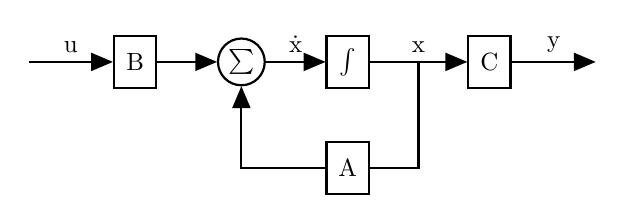
\begin{tikzpicture}[ auto,
                       thick,                         %<--setting line style
                       node distance=1.5cm,             %<--setting default node distance
                       scale=.9,                     %<--|these two scale the whole thing
                       every node/.style={scale=.9}, %<  |(always change both)
                       >=triangle 45 ]                %<--sets the arrowtype
    
    \draw%-----------------------------------------------------------------------------------------
    	%Drawing Input/Output:
    	node[shape=coordinate][](input1) at (0,0){}
    	node[shape=coordinate][](output1) at (8,0){}
     	%Drawing the Equation Blocks:   	
      	node(A) at (4.5,-1.5) [block] {A} 
     	node(B) at (1.5,0) [block] {B}
     	node(C) at (6.5,0) [block] {C}
%      	node(D) at (4.5,1.5) [block] {D}  
	    node(int) at (4.5,0) [block] {\si{\int}}  
    	%Drawing the Sumation Blocks:	    	 	
    	node(sum1) [sum, right of = B] {\si{\sum}}
%    	node(sum2) [sum, right of = C] {\si{\sum}}
    	%Drawing the Feedback/Feedforward Nodes:    	
    	node[shape=coordinate][](FeedforwardNode) at (0.75,0){}
    	node[shape=coordinate][](FeedbackNode) at (5.5,0){}  	
    	     
    ;%---------------------------------------------------------------------------------------------
   
    %Joining the Blocks
  	\draw[->](input1) -- node {u}(B);
  	\draw[->](B) -- node {}(sum1);
  	\draw[->](sum1) -- node {\si{\dot x}}(int);  	
  	\draw[->](int) -- node {x}(C);
  	\draw[->](C) -- node {y}(output1);
  	
%  	\draw[->](FeedforwardNode) |- node{} (D);
%  	\draw[->](D) -| node{} (sum2);

  	\draw[-] (FeedbackNode) |- (A);
  	\draw[->] (A)   -| (sum1);

    %Drawing node(s) with \textbullet
    \draw%--------------------------------------------------------------
%      node at (input1)  [shift={(-0.04, -0.04 )}] {\large \textbullet}
    	% node at (output1) [shift={( 0.008, -0.02 )}] {\textbullet}
    ;%------------------------------------------------------------------
  \end{tikzpicture}
  	\end{textblock*}
  }
  \only<1-2>
    {
    \tikz[overlay,xshift=7.5em,yshift=-16ex]{\draw node {
        \begin{minipage}{0.01\linewidth}
         	\begin{flalign}
         		\vec{x} = 
         		\begin{bmatrix}
         			\theta_F \\
         			\dot{\theta}_F \\ 
         			\dot{\theta}_w \\
         		\end{bmatrix}	\textbf{,}\ \nonumber
         	\end{flalign}  
        \end{minipage}
        %\hspace{0.03\linewidth}
        \begin{minipage}{0.01\linewidth}
         	\begin{flalign}
         		\vec{y} = 
         		\begin{bmatrix}
         			\theta_F \\
         			\dot{\theta}_w \\
         		\end{bmatrix}	\textbf{,}\ \nonumber
         	\end{flalign}
        \end{minipage}
        %\hspace{0.03\linewidth}
        \begin{minipage}{0.01\linewidth}
         	\begin{flalign}
         		\vec{u}= 
         		\begin{bmatrix}
         			\tau_m\\
         		\end{bmatrix}	\nonumber
         	\end{flalign}
      \end{minipage}
    };}
  }   
\end{frame}

%---------------------------------------------------------------------------------
\subsection{Controller Design}%---------------------------------------------------
%---------------------------------------------------------------------------------
\begin{frame}{State Space}{Controller Design}
  \begin{itemize}
    \item Eigenvalues of \si{(\vec{A} - \vec{B} \vec{K})}
    \item Pole placement
  \end{itemize}

  \begin{displaymath}
  	\hspace{-5cm}\si{\vec{\dot{x}}(\vec{t}) = (\vec{A}-\vec{B}\vec{K}) \cdot \vec{x}(\vec{t})} \nonumber
  \end{displaymath}
  
  \begin{figure}[H]
      \centering
      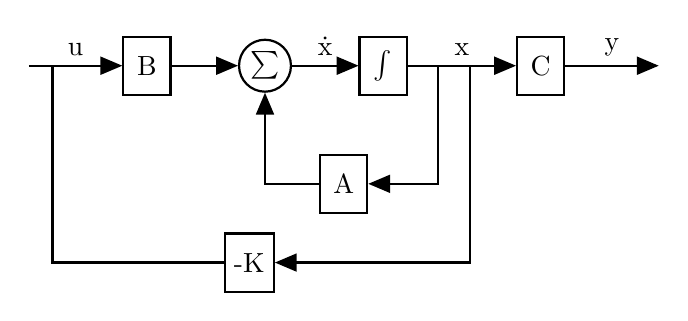
\begin{tikzpicture}[ auto,
					thick,                         %<--setting line style
					node distance=1.5cm,             %<--setting default node distance
					scale=1,                     %<--|these two scale the whole thing
					every node/.style={scale=1}, %<  |(always change both)
					>=triangle 45 ]                %<--sets the arrowtype

	\draw%-----------------------------------------------------------------------------------------
	%Drawing Input/Output:
	node[shape=coordinate][](input1) at (0,0){}
	node[shape=coordinate][](inputFeedback) at (.3,0){}
	node[shape=coordinate][](output1) at (8,0){}
	%Drawing the Equation Blocks:   	
	node(A) at (4,-1.5) [block] {A} 
	node(B) at (1.5,0) [block] {B}
	node(C) at (6.5,0) [block] {C}
	node(int) at (4.5,0) [block] {\si{\int}} 
	node(K) at (2.8,-2.5) [block] {-K}	
	%Drawing the Sumation Blocks:	    	 	
	node(sum1) [sum, right of = B] {\si{\sum}}
	%Drawing the Feedback/Feedforward Nodes:    	
	node[shape=coordinate][](FeedbackNode) at (5.2,0){}  	
	node[shape=coordinate][](FeedbackNode2) at (5.6,0){} 
	
	;%---------------------------------------------------------------------------------------------

	%Joining the Blocks
	\draw[->](input1) -- node {u}(B);
	\draw[->](B) -- node {}(sum1);
	\draw[->](sum1) -- node {\si{\dot x}}(int);  	
	\draw[->](int) -- node {x}(C);
	\draw[->](C) -- node {y}(output1);

	\draw[->] (FeedbackNode) |- (A);
	\draw[->] (A)   -| (sum1);
	
	\draw[->] (FeedbackNode2) |- (K);
	\draw[-] (K)   -| (inputFeedback);

	%Drawing node(s) with \textbullet
	\draw%--------------------------------------------------------------
%	node at (input1)  [shift={(-0.08, -0.02 )}] {\large \textbullet}
	% node at (output1) [shift={( 0.008, -0.04 )}] {\textbullet}
	;%------------------------------------------------------------------

\end{tikzpicture}
  \end{figure}
\end{frame}

\begin{frame}{State Space}{Controller Design}
  \begin{itemize}
    \item Controller reacting to disturbance
    \item Different pole placements
    \item The yellow was chosen
  \end{itemize}
  \vspace{.5cm}
  \hspace{0.03\linewidth}
  \begin{minipage}{\linewidth}
   	\begin{minipage}{0.45\linewidth}
   		\begin{figure}[H]
   			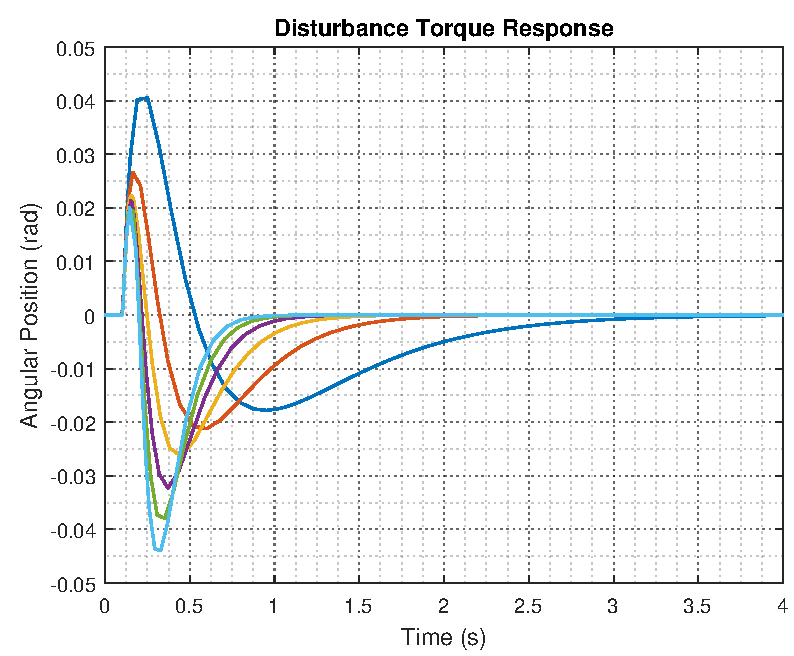
\includegraphics[scale=.35]{Pictures/disturbanceStateSpace}
   			\centering
   		\end{figure}
   	\end{minipage}
   	\hspace{0.03\linewidth}
   	\begin{minipage}{0.45\linewidth}
   		\begin{figure}[H]
   			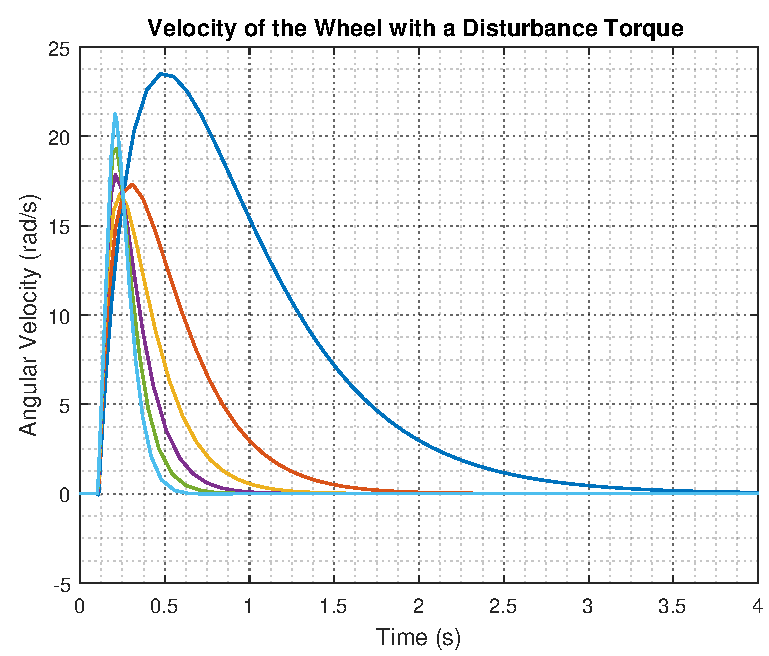
\includegraphics[scale=.35]{Pictures/disturbanceStateSpaceWheel}
   			\centering
   		\end{figure}
   	\end{minipage}
  \end{minipage}
\end{frame}

%---------------------------------------------------------------------------------
\subsection{Controller Analysis}%-------------------------------------------------
%---------------------------------------------------------------------------------

\begin{frame}{State Space}{Controller Analysis}
    \begin{minipage}{\linewidth}
    	\begin{minipage}{0.4\linewidth}
    		\begin{figure}
    			\includegraphics[scale=.35]{Pictures/positionRLTest}
    			\centering
    		\end{figure}
    	\end{minipage}
    	\hspace{0.1\linewidth}
    	\begin{minipage}{0.45\linewidth}
    		\begin{figure}[H]
    			\includegraphics[scale=.35]{Pictures/wheelRLTest}
    			\centering
    		\end{figure}
    	\end{minipage}
    \end{minipage}
  \vspace{.5cm}
  \begin{minipage}{\linewidth}
   	\begin{minipage}{0.45\linewidth}
   		\begin{figure}[H]
   			\includegraphics[scale=.35]{Pictures/positionSSTest}
   			\centering
   		\end{figure}
   	\end{minipage}
   	\hspace{0.03\linewidth}
   	\begin{minipage}{0.45\linewidth}
   		\begin{figure}[H]
   			\includegraphics[scale=.35]{Pictures/wheelSSTest}
   			\centering
   		\end{figure}
   	\end{minipage}
  \end{minipage}
\end{frame}


% %---------------------------------------------------------------------------------
% \subsection{Animation Test}%------------------------------------------------------
% %---------------------------------------------------------------------------------

% \begin{frame}{Animation Test}{wooohooo}
%   \transduration<0-19>{1.5}
%   \multiinclude[format=png, graphics={width=\textwidth}]{Pictures/optJoinedFit/cost}
%   %\animategraphics[autoplay,loop,width=\linewidth]{1}{Pictures/cost-}{0}{19}
% \end{frame}
	%%%%%%%%%%%%%%%%%%%%%%%%%%%%%%%%%%% NAME %%%%%%%%%%%%%%%%%%%%%%%%%%%%%
%%%%%%%%%%%%%%%%%
\section{Complementary Filter}
%%%%%%%%%%%%%%%%%

%%%%%%%%%%%%%%%%
\subsection{Gyroscope}
\begin{frame}{Complementary Filter}{Gyroscope}
A gyroscope measures angular velocity by integrating small intervals to find the orientations.
\begin{figure}
	\centering
	\includegraphics[scale=0.4]{Pictures/angleGyro.pdf}
\end{figure}

The problems with the gyroscope are:
	\begin{itemize}
		\item {By integrating, the error is accumulating over time.}
		\item {The gyroscope may experiencing drifting errors from small and slow movement.}
	\end{itemize}
\end{frame}
%%%%%%%%%%%%%%%
%%%%%%%%%%%%%%%%
\subsection{Accelerometers}
\begin{frame}{Complementary Filter}{Accelerometers}
An accelerometer measures inertial force, such as gravity and relies on a constant gravitational pull with respect to the Earth, and the calculations orientation can be found.
\begin{figure}
	\centering
	\includegraphics[scale=0.4]{Pictures/angleAcc.pdf}
\end{figure}

The problems for accelerometers are:
\begin{itemize}
	\item {They are very sensitive to mechanical noise and vibrations.}
\end{itemize}
\end{frame}
%%%%%%%%%%%%%%%%
%%%%%%%%%%%%%%%%
\subsection{Sensor Fusion}
\begin{frame}{Complementary Filter}{Sensor Fusion}
Data from accelerometers and gyroscopes can be combined for a better estimate of orientation than using only accelerometer data.\linebreak

The combined data can help fix noise and drift error. A method is to use a complementary filter.
\begin{figure}
	\centering
	\includegraphics[scale=0.5]{Pictures/Complementary.pdf}
\end{figure}
Complementary filter advantages is:
\begin{itemize}
	\item {Fast estimates of angle and much less lag than low-pass filter alone.}
	\item {Not very processor-intensive.}
\end{itemize}
\end{frame}
%%%%%%%%%%%%%%%%
%%%%%%%%%%%%%%%%
\subsection{Cut-off Frequency}
\begin{frame}{Complementary Filter}{Cut-off Frequency}
High pass and low pass filters with the same cut-off frequency. 
\begin{figure}
	\centering
	\includegraphics[scale=0.5]{Pictures/bodeFilters.pdf}
\end{figure}
The summation of both cut-off frequency gives a gain of 1.
\end{frame}
%%%%%%%%%%%%%%%%
%%%%%%%%%%%%%%%%
\subsection{Compare Results}
\begin{frame}{Complementary Filter}{Compare Results}
The complementary filter compared with the data from the potentiometer.
	\begin{figure}
		\centering
		\includegraphics[scale=0.5]{Pictures/filterSensTool.pdf}
	\end{figure}
The two measurements match closely.
\end{frame}
%%%%%%%%%%%%%%%%
%%%%%%%%%%%%%%%%%%%%%%%%%%%%%%%%%% NAME %%%%%%%%%%%%%%%%%%%%%%%%%%%%%
%%%%%%%%%%%%%%%%
\section{Acceptance Test}
%%%%%%%%%%%%%%%%

%%%%%%%%%%%%%%%%
\subsection{Requirements Test}

\begin{frame}{Acceptance Test}{Requirements Test}
- The Cubli should be able to balance starting from an unstable equilibrium position and null velocity.\linebreak

\begin{minipage}{\linewidth}
	\begin{minipage}{0.45\linewidth}
		\begin{figure}[H]
			\centering
			\includegraphics[scale=.345]{Pictures/testReq1}
		\end{figure}
	\end{minipage}
	\hspace{0.03\linewidth}
	\begin{minipage}{0.45\linewidth}
		\begin{figure}[H]\vspace{0mm}
			\centering
			\includegraphics[scale=.345]{Pictures/testReq1_IMU}
		\end{figure}
	\end{minipage}
\end{minipage}\linebreak

Angular position of the frame, when starting from equilibrium position.
	\begin{itemize}
		\item {Measured with the potentiometer.}
		\item {Calculated with the complementary filter.}
	\end{itemize}
	 
 
\end{frame}
%%%%%%%%%%%%%%%%
%%%%%%%%%%%%%%%%
\subsection{Requirements Test}

\begin{frame}{Acceptance Test}{Requirements Test}
- The prototype should be able to balance around 0 rad, even though the angle of inclination of the baseplate is changed within a reasonable range, using internally mounted sensors.
	
\begin{figure}
	\centering
	\includegraphics[scale=0.40]{Pictures/testReq2.pdf}
\end{figure}
Position of the frame which does not depend on the angle of the baseplate.
\end{frame}
%%%%%%%%%%%%%%%%

%%%%%%%%%%%%%%%%%%%%%%%%%%%%%%%%%%% NAME %%%%%%%%%%%%%%%%%%%%%%%%%%%%%
%%%%%%%%%%%%%%%%
\section{Conclusion}
%%%%%%%%%%%%%%%%

%%%%%%%%%%%%%%%%
\subsection{Conclusion}

\begin{frame}{Conclusion}{Cubli}
Maximum recovery angle while disturbances is applied:
	\begin{itemize}
		\item {The controller is capable of recovering from \si{0,08\ rad} (\si{4,58^\circ}).}
		\item {The controller is not able to recover from greater angle due to overshoot.}\linebreak
	\end{itemize}
	
Maximum catching angle with no initial velocity of the wheel is \si{0,2024\ rad} (\si{11,59^\circ}):
	\begin{itemize}
		\item {The controller is capable of catching the frame when it starts from \SI{-0,17}{rad}  (\si{-9,74^\circ}).}
		\item {The controller is not able to recover from greater angle due to overshoot.}\linebreak
	\end{itemize}
It is not possible to catch and balance the system in equilibrium position from a  greater angle than \SI{-0,17}{rad}  (\si{-9,74^\circ}).\linebreak
\end{frame}
%%%%%%%%%%%%%%%%
%%%%%%%%%%%%%%%%
\subsection{Conclusion}

\begin{frame}{Conclusion}{Cubli}
	Improving the system:
	\begin{itemize}
		\item {Measurements of the IMU could be improved by moving the sensor.}
		\item {Fusing Sensor data from IMU using a different filter type.}\linebreak
	\end{itemize}
	
It was also a requirement to be able to:
	\begin{itemize}
		\item {Keep it in upright position.}
		\item {Change the angle of the baseplate.}\linebreak
	\end{itemize}
	
In conclusion:
	\begin{itemize}
		\item {The state space controller constructed has been tested successfully within the requirements.}
	\end{itemize}
\end{frame}
%%%%%%%%%%%%%%%%
		
		
	\end{document}

